%
% File naaclhlt2015.tex
%
\documentclass[11pt,letterpaper]{article}
\usepackage{naaclhlt2015}
\usepackage{times}
\usepackage{latexsym}
\setlength\titlebox{6.5cm}    % Expanding the titlebox
\usepackage{amsmath}
\usepackage{multirow}
\usepackage{url}
\usepackage{graphicx}
\usepackage{hhline}

\usepackage{algorithm}
\usepackage[noend]{algpseudocode}
\usepackage{comment}
\makeatletter
\def\BState{\State\hskip-\ALG@thistlm}
\makeatother
 %\usepackage{algolyx}
%\setotherlanguage{urdu}
%\newfontfamily\urdufont[Script=Arabic,Language=Urdu,Scale=1.5]{Amiri}
%\usepackage{footnotebackref}[2012/07/01]



\DeclareMathOperator*{\argmax}{arg\,max}
\setlength\titlebox{6.5cm}    % Expanding the titlebox
%Quality Control vs. Cost Optimization in Crowdsourcing Translation%
\title{Cost Optimization in Crowdsourcing Translation:\\ Low cost translations made even cheaper}

\author{First Author \\
  Affiliation / Address line 1 \\
  Affiliation / Address line 2 \\
  Affiliation / Address line 3 \\
  {\tt email@domain} \\\And
  Second Author \\
  Affiliation / Address line 1 \\
  Affiliation / Address line 2 \\
  Affiliation / Address line 3 \\
  {\tt email@domain} \\}

\date{}

\begin{document}
\maketitle
\begin{abstract}
Crowdsourcing makes it possible to create translations at low cost. We proposed two mechanisms to make this process even cheaper while maintaining high translation quality.
First, we develop a translation reducing method.  We train a linear model to evaluate the translation quality on a sentence-by-sentence basis, and fit a threshold between acceptable and unacceptable translations.   Unlike past work, which always paid for a fixed number of translations of each source sentence and then chose the best from among them, we can decide after seeing a single translation whether it is good enough or not. Our model based selection allows us to reduce cost by reducing the number of redundant translations that we solicit. 
Second, we introduce a translator reducing method that allows us to reduce cost by quickly identifying bad translators after they have translated only a few sentences.  This allows us to rank translators, so that we only re-hire good translators and so that we can select the best translations from among good candidates. 
%Additionally, we show that costs associated with gold standard calibration data created by professional translators can be reduced by using single reference instead of multiple references. 
%Besides, we reduce the cost for professional translations by reducing the number of references to calibrate each non-professional translation. 
 \end{abstract}

\section{Introduction}

Crowdsourcing is a promising new mechanism for collecting large volumes of annotated data at low cost.  %Platforms like Amazon Mechanical Turk (MTurk) provide researchers with access to large groups of people, who can complete `human intelligence tasks' that are beyond the scope of current artificial intelligence. 
%Since statistical natural language processing benefits from increased amounts of labeled training data, 
Many NLP researchers have focused on creating speech and language data through crowdsourcing (for example,  \newcite{snow2008}, \newcite{callison-burch-dredze2010} and others).  One NLP application that has been the focus of crowdsourced data collection is statistical machine translation (SMT) which requires large bilingual sentence-aligned parallel corpora to train translation models.  Crowdsourcing's low costs has made it possible to hire people to create sufficient volumes of translation in order to train SMT systems (for example,   \newcite{zbib2013systematic},  \newcite{zbib2012machine},  \newcite{post2012constructing}, \newcite{ambati2010can}).

However, crowdsourcing is not perfect, and one of its most pressing challenges is how to ensure the quality of the data that is created by it.  Unlike in more traditional employment scenarios, where annotators are pre-vetted and their skills are clear, in crowdsourcing very little is known about the annotators.  They are not professional translators, and there are no built-in mechanisms for testing their language skills.  They complete tasks without any oversight. Thus, translations produced via crowdousrcing may be low quality.
Previous work has addressed this problem, showing that non-professional translators hired on Amazon Mechanical Turk (MTurk) can achieve professional-level quality, by soliciting multiple translations of each source sentence and then choosing the best translation \cite{zaidan-callisonburch:2011:ACL-HLT2011a}.

In this paper we focus on a different aspect of crowdsourcing from \newcite{zaidan-callisonburch:2011:ACL-HLT2011a}.  We attempt to achieve the same high quality while {\bf minimizing the associated costs}.  
%We reduce the costs associated with non-professional translations. 
We propose two complementary methods:
(1) We reduce the number of translations that we solicit for each source sentence. Instead of soliciting a fixed number of translations for each foreign sentence, we stop soliciting translations after we get an acceptable one.  We do so by building models to distinguish between acceptable translations and unacceptable ones. (2) We reduce the number of workers we hire, and retain only high quality translators by quickly identifying and filtering out workers who produce low quality translations. 
  

Our work stands in contrast with  \newcite{zaidan-callisonburch:2011:ACL-HLT2011a} who always solicited and paid for a fixed number of translations of each source segment, and who had no model of annotator quality. 
 
 In this paper we demonstrate that
 \begin{itemize}
 \item Our model can predict whether a given translation is acceptable with high accuracy, substantially reducing the number of redundant translations needed for every source segment.
 \item Workers can be ranked by their quality with high correlation against a gold standard ranking, using linear regression and a variety of features, or initially testing them using a small amount of calibration data with known professional translations.
 \item This ranking can be established after observing very small amounts of data (reaching $\rho$ of 0.91 after seeing the translations of only 20 sentences from each worker). Therefore, bad workers can be filtered out quickly.
 
 \item We can achieve a similar BLEU score as \newcite{zaidan-callisonburch:2011:ACL-HLT2011a} at half the cost using our cost optimizing methods.
 % and at 60\% of the non-professional translations' cost using model selection method.  
 \end{itemize} 
 
\section{Problem Setup}

We start with a corpus of source sentences to be translated, and we may solicit one or more translation for every sentence in the corpus.  Our goal is to assemble a single high quality translation for each source sentence while minimizing the associated cost. 

We study the data collected by \newcite{zaidan-callisonburch:2011:ACL-HLT2011a} through Amazon's Mechanical Turk. 
They hired Turkers to translate 1792 Urdu sentences 
from the  2009 NIST Urdu-English Open Machine Translation Evaluation set\footnote{LDC Catalog number LDC2010T23}. A total of 52 Turkers contributed translations. Turkers also filled out a survey about their language skills and their countries of origin. Each Urdu sentence was translated by 4 non-professional translators (the Turkers) and 4 professional translators hired by the LDC. The cost of for non-professional translation is  \$0.10 per sentence and the cost of professional translation is approximately \$0.30 per word (or \$6 per sentence, since they are 20 words long on average). 

Following \newcite{zaidan-callisonburch:2011:ACL-HLT2011a}, we use BLEU \cite{papineni2002bleu} to gauge the quality of human translations.  We can compute the expected quality of professional translation by comparing each of the professional translators against the other 3.  This results in an average BLEU score of  42.38.  By comparison, the Turker translations score only 28.13 on average. Zaidan and Callison-Burch trained a MERT model to select one non-professional translation out of the four and pushed the quality of crowdsourcing translation to 39.06, closer to the expected quality of professional translation. They used a small amount of professional translations (10\%) as calibration data to estimate the goodness of the non-professional translation. The component costs of their approach are the 4 non-professional translations for each source sentence, and the professional translations for the calibration data.

Although Zaidan and Callison-Burch demonstrated that non-professional translation was significantly cheaper than professionals, we are interested in further reducing the costs.  This plays a role if we would like to assemble a large enough parallel corpus (on the order of millions of pairs of sentences) to train a statistical machine translation system. 
% \cite{ambati2010can,post2012constructing,zbib2012machine,zbib2013systematic}
Here, we introduce several methods for reduce the number of non-professional translations  while still maintaining high quality. 
\section{Estimating Translation Quality}
We use a linear regression model\footnote{We used WEKA package: \url{http://www.cs.waikato.ac.nz/ml/weka/}} to predict a quality score ($ score(t) \in R$) for an input translation $t$.
%\begin{align*}
\[ score(t) = \vec{w}  \cdot \vec f(t) \]
  %\end{align*}
  where $\vec{w}$ is the associated weight vector and $\vec f(t)$ is the feature vector of the translation $t$. 

We replicate the feature set used by \newcite{zaidan-callisonburch:2011:ACL-HLT2011a} in their MERT model:

\begin{itemize}
\item  Sentence-level features: 9 features based on language model, sentence length, edit distance to other translations. 
\item Worker-level features: 15 features based on worker's language ability, location and average sentence-level scores.
\item Ranking features: 3 features based on the judgments of monolingual English speakers ranking the translations from best to worst.
\item Calibration features: 1 feature based on the average BLEU score of translations provided by the same worker, which is computed against professional references.
%\item Bilingual features: 1 feature based on the word alignment probabilities according. 
\end{itemize}


We additionally introduce a new bilingual feature based on IBM Model 1. We align words between each candidate translation and its corresponding source sentence. The bilingual feature for a translation is the average of its alignment probabilities. In Figure \ref{biexample1}, we show how the bilingual feature allows us to distinguish between a valid translation (top) and an invalid/spammy translation (bottom).

\begin{figure}[h!]
  \centering
  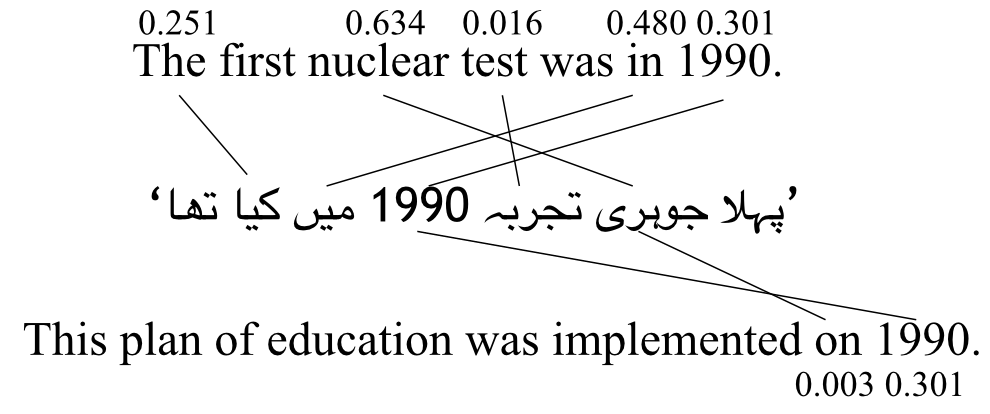
\includegraphics[width=\linewidth]{bilingualexample/example.png}
  \caption{Example bilingual feature for two crowdsourced translations for a sentence in Urdu. The numbers are alignment probabilities for each aligned word. The bilingual feature is the average of these probabilities, thus 0.240 for the good translation and 0.043 for the bad translation. Some words are not aligned if potential word pairs don't exist in corpus.
}
    \label{biexample1}
\end{figure}

%\newcite{zaidan-callisonburch:2011:ACL-HLT2011a} used all 4 professional translations in computing the calibration features and training labels. We will show in the experiments that using \textbf{only one} professional translation as reference is as sufficient. 

\section{Reducing the Number of Translations}
The first mechanism that we introduce to optimize cost is one that reduces the number of translations.  Our goal is to recognize when we have got a good translation of a source sentence and to immediately stop purchasing additional  translations of that sentence.  The crux of this method is to decide whether a translation  is `good enough,' in which case we do not gain any benefit from  paying for another redundant translation.  

Our translation reduction method allows us to set an empirical definition of `good enough'.  We introduce a parameter  of the model  ($\delta$) that allows us to set how much degradation in translation quality is allowable, when we compare against selecting the best translation from the full set of redundant translations.  For instance, we may fix $\delta$ at 95\%, meaning that the BLEU score should not drop below 0.95 of the estimated BLEU score using the full set of non-professional translations.   We train a model to search for a threshold between acceptable and unacceptable translations ($\theta$) for a specific value of $\delta$. 

For a new translation, our model scores it, and if its score is higher than $\theta$, then we do not solicit another translation. Otherwise, we continue to solicit translations.  Algorithm \ref{modelselection} details the process of model training and searching for $\theta$. 

%%%%%

\begin{algorithm} [h!]
\caption{}\label{modelselection}
\textbf{Input}: $\delta$,  the allowable deviation from the expected upper bound on BLEU score (using all redundant translations); a training set $S = \{\vec f^{s}_{i,j},y^{s}_{i,j})_{i=1..n}^{j=1..4}\}$ and a validation set $V = \{(\vec f^{v}_{i,j},y^{v}_{i,j})_{i=1..n}^{j=1..4}\}$ where $\vec f_{i,j}$ is the feature vector for $t_{i,j}$ which is the $jth$ translation of the source sentence $s_{i}$ and $y_{i,j}$ is the label for $\vec f_{i,j}$.\\
\textbf{Output}: $\theta$, the threshold between acceptable and unacceptable translations; $\vec{w}$, a linear regression model parameter. 
\begin{algorithmic}[1]
\State \textbf{initialize} $\theta \leftarrow 0$,$\vec{w}\leftarrow \emptyset$ 
\State $\vec{w'}\leftarrow$ train a linear regression model on T
\State $maxbleu \leftarrow$ select best translations for each $s_i \in T$ based on the model parameter $\vec{w'}$ and record the highest model predicted BLEU score
\State $\alpha \leftarrow$ set an upper-bound BLEU score empirically
\While {$\theta \neq maxbleu $} 
\For {$i \leftarrow 1$ to $n$}
\For {$j \leftarrow 1$ to $4$}
\If {$\vec{w'}\cdot \vec f^v_{i,j} > \theta \wedge j < 4 $}
             select $t^{v}_{i,j}$ for $s_i$ and \textbf{break}
\EndIf
\If {$ j == 4 $} select $t^{v}_{i,j}$ for $s_i$
\EndIf
\EndFor
\EndFor
\State $q \leftarrow$ calculate translation quality for V
\If {$q > \delta \cdot \alpha$} \textbf{break}
\Else \text{  } $\theta = \theta + stepsize$
\EndIf
\EndWhile
\State $\vec {w} \leftarrow$ train a linear regression model on $S \cup V$
\State \textbf{Return}: $\theta$ and model parameter $\vec{w}$
%\EndProcedure
\end{algorithmic}
\end{algorithm}


%%%%%%

%
%\begin{algorithm} [h!]
%\caption{}\label{modelselection}
%\textbf{Input}: $\delta$, the allowable deviation from the expected upper bound on BLEU score (using all redundant translations); $S = \{(x^{s}_{i,j},y^{s}_{i,j})^{j=1...4}_{i = 1...n}\}$ and a validation set $V = \{(x^{v}_{i,j},y^{v}_{i,j})_{j=1}^{4}\}_{i=1}^n$ where $x_{i,j}$ is the feature vector for the jth translation of the source sentence $s_{i}$ and $y_{i,j}$ is the label for $x_{i,j}$.\\
%\textbf{Output}: $\theta$, the threshold between acceptable and unacceptable translations; m(x), a linear regression model. 
%\begin{algorithmic}[1]
%\State \textbf{initialize} $\theta \leftarrow 0$,$m(x)\leftarrow \emptyset$ 
%\State $m'(x)\leftarrow$ train a linear regression model on T
%\State $maxbleu \leftarrow$ use $m'(x)$ select best translations for each $s_i \in T$ and record the highest model predicted BLEU score
%\State $upperbound \leftarrow$ set an upper-bound BLEU score empirically
%\While {$\theta \neq maxbleu $} 
%\For {$i \leftarrow 1$ to $n$}
%\For {$j \leftarrow 1$ to $4$}
%\If {$m'(x^{v}_{i,j}) > \theta \wedge j < 4 $}
%             select $x^{v}_{i,j}$ for $s_i$ and \textbf{break}
%\EndIf
%\If {$ j == 4 $} select $x^{v}_{i,j}$ for $s_i$
%\EndIf
%\EndFor
%\EndFor
%\State $q \leftarrow$ calculate translation quality for V
%\If {$q > \delta \cdot upperbound$} \textbf{break}
%\Else \text{  } $\theta = \theta + stepsize$
%\EndIf
%\EndWhile
%\State $m \leftarrow$ train a linear regression model on $S \cup V$
%\State \textbf{Return}: $\theta$ and model $m(x)$
%%\EndProcedure
%\end{algorithmic}
%\end{algorithm}
%

\subsection{Experiment}
 We divide data into a training set (10\%), a validation set (10\%) and a test set (80\%). 
We use the validation set to establish an upper-bound BLEU ($\alpha$) is set to be 0.4013 empirically. 
We then vary the value of $\delta$ from 90\% to 100\%, and sweep values of $\theta$ by incrementing it in step sizes of 0.01.
We report results on based on a five-fold cross validation, rotating the training, validation and test sets.

\subsubsection{Baseline and upper bound} 
The baseline selection method of randomly picking one translation for each source sentence achieves a BLEU score of 29.56. To establish an upper bound of the translation quality, we perform an oracle experiment which operates on full set of redundant translations and selects best translations among them  by a linear regression model trained on the union set of training and validating data. We get a surprisingly high BLEU score of 40.13.

\subsubsection{Translation reducing method} Table \ref{orderanother} shows the results for translation reducing method. We get comparable translation quality against our competing method with a much lower cost. If we set $\delta$ as 0.95, comparing two method, the difference in translation quality is 2.09 and for each source sentence, we almost avoid paying two redundant translations on average.
% The cost is:
% \begin{align*}
%  C& = \frac{\alpha}{4} \cdot \frac{2}{10} N_{p}\cdot C_{p}  + \frac{3.12}{4} \beta\cdot \frac{8}{10} N_{np} \cdot C_{np}\\
%   & = 2,608.43 (\$)
% \end{align*}
% which is 52\% of the original total cost and  28\% of the cost of our competing method.
 \begin{table}[h]
 \center
\begin{tabular}{c|c|c}
\hline
$\delta$(\%) & BLEU Score & \# of Trans. \\ \hhline{===}
90    & 36.26      & 1.63            \\
91    & 36.66      & 1.69             \\
92    & 36.93      & 1.78             \\
93    & 37.23      & 1.85             \\
94    & 37.48      & 1.93             \\
95    & 38.05      & 2.21             \\
96    & 38.16      & 2.30             \\
97    & 38.48      & 2.47             \\
98    & 38.67      & 2.59             \\
99    & 38.95      & 2.78             \\
100   & 39.54      & 3.18             \\ \hline
\end{tabular}
\caption{The relation among the $\delta$ (the allowable deviation from the expected upper bound on BLEU score),the BLEU score for translations selected by models from partial sets and the averaged size of translation candidates set for each source sentence (\textit{\# of Trans}).  }
    \label{orderanother}
\end{table}
% \begin{table*}[t]
% \center
%\begin{tabular}{|c|c|c|c|}
%\hline
%Source                                   & References                         & Translations                         & Quality \\ \hline
%\multirow{4}{*}{فرانس کی تجویز کی حمایت} & Support of France's Recommendation & France has supported the proposal.   & 0.342   \\ \cline{2-4} 
%                                         & Support for the Proposal of France & Supporting the French proposal       & 0.630   \\ \cline{2-4} 
%                                         & French Proposal Endorsed           & France suggestion was appriciatable. & -0.014  \\ \cline{2-4} 
%                                         & French Proposal Supported          & defending the thinking of France.    & 0.269   \\ \hline
%\end{tabular}
%\caption{An example showing how to reduce redundant translations using the  model and the threshold. For each source sentence, we solicit 4 references and 4 non-professional translations. The value of 'Quality' is the \textbf{ model predicted score} for each translation which is different from the BLEU score. In this example, \textit{delta} is \%95, and the threshold telling apart acceptable and unacceptable translations is 0.35. Translations listed from top to the bottom are in the chronological order from the earliest submitted one to the latest submitted one. Since the first translation's quality value is lower that the threshold, we need to solicit another one.  Knowing that the second translation's quality value is higher than the threshold,  we stop soliciting other translations for this source sentence so that we avoid collect redundant translations and reduce cost.}
%\label{texample}
%\end{table*}


\section{Choosing Better Translators}

The second mechanism that we use to optimize cost is to reduce the number of non-professional translators that we hire.  Our goal is to quickly identify whether Turkers are good or bad translators, so that we can continue to hire only the good translators and stop hiring the bad translators after they are identified as such. 
%
Before presenting our method, we first demonstrate that Turkers produce consistent quality translations over time.

%reducing the number of translators by quickly identifying bad workers and filtering them out. We achieve high translation quality and avoid hiring bad workers continually after having detected their bad performance.

\subsection{Turkers' behavior in translating sentences}



\begin{figure}[h!]
  \centering
  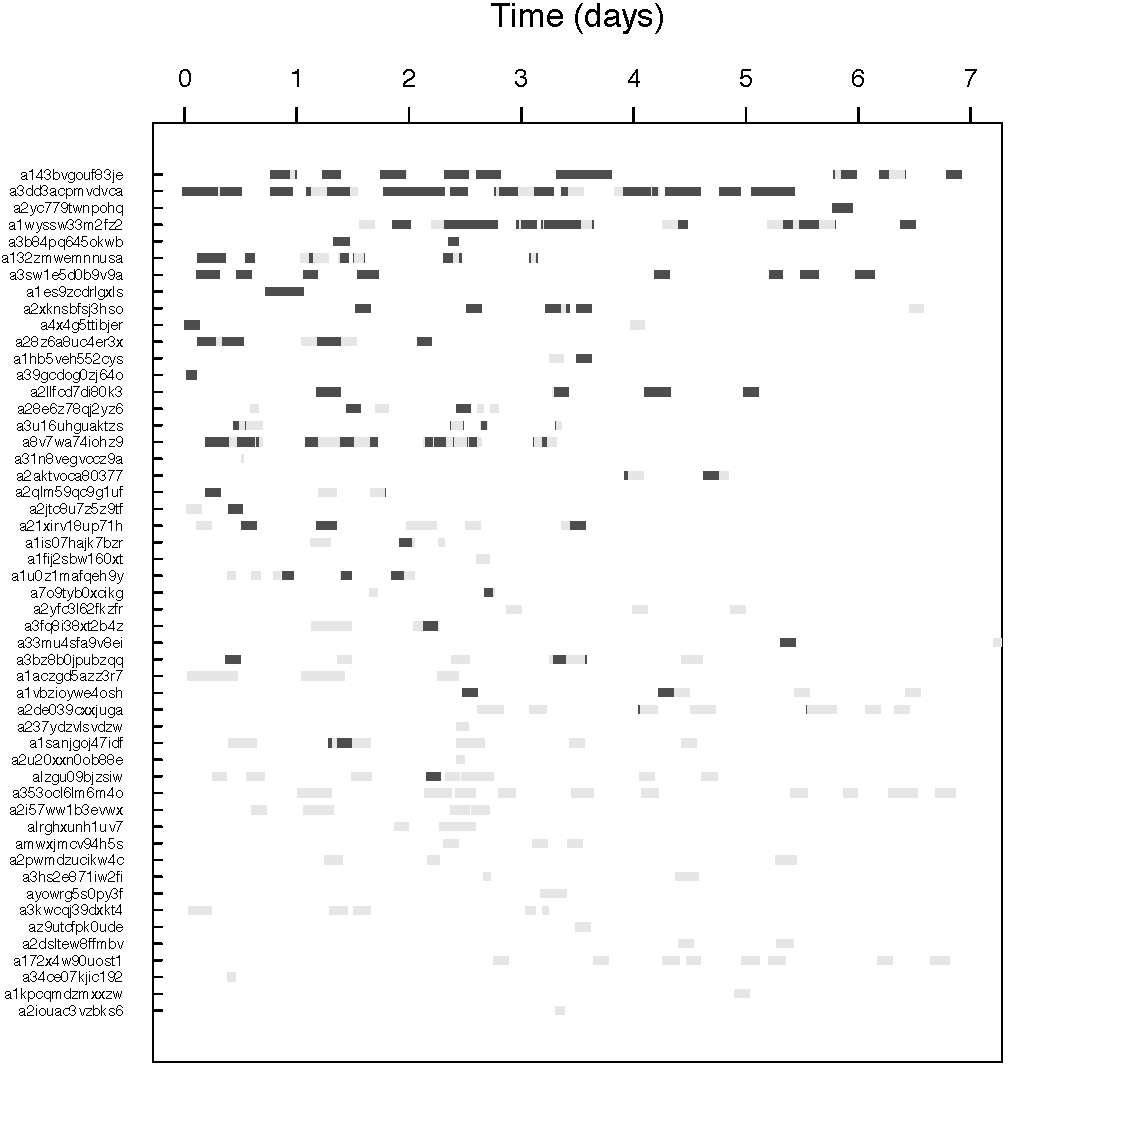
\includegraphics[width=\linewidth]{WorkerPerf/wp.pdf}
  \caption{A time-series plot of all of the translations produced by Turkers (identified by their WorkerID serial number). Turkers are sorted with the best translator at the top of the y-axis. Each tick represent a single translation and dark color means better quality.
}
    \label{fworkerperf}
\end{figure}

Do Turkers produce good (or bad) translations consistently or not? Are some Turkers  consistent and others not? We used the professional translations as a gold-standard to analyze the individual Turkers, and we found that most Turkers' performance stayed surprisingly consistent over time. 

Figure \ref{fworkerperf} illustrates the consistency of workers' quality by plotting quality of their individual translations on a timeline. The translation quality is computed based on the BLEU against professional translations. Each tick represent a single translation and depicts the BLEU score using two colors. The tick is black if its BLEU score is higher than the median and it is light grey otherwise. Good translators tend to produce consistently good translations and bad workers rarely produce good translations.

%Since workers' performance is consistent, workers' rankings are sufficiently accurate to reflect the quality of translations provided by them and we can select the translation which is provided by the worker with the best rank. We propose two approaches to rank workers from a small portion of work they submitted, filter out bad workers and select the best translation from translations provided by  surviving workers.
\subsection{Ranking Evaluation}
We compare our ranking of workers with gold standard ranking and calculate the correlation score. Since workers translated different number of sentences, we set a weight to each worker using the number of translations he/she submitted to represent his/her importance. Taking the importance of workers into consideration when calculating the correlation, we use the weighted Pearson correlation algorithm\footnote{http://en.wikipedia.org/wiki/Pearson\_product-moment\_correlation\_coefficient\# cite\_note-22} in our case.
Given two ranking list \textit{x} and \textit{y} showing workers' ranks and the weight vector \textit{w}, the weighted correlation $corr$ can be calculated as:
\begin{gather*}
 m(x;w)  =  \frac{\sum_{i} w_i x_i}{\sum_i w_i} \\
 cov(x,y;w)  = \frac{\sum_i w_i (x_i - m(x;w))(y_i - m(y;w))}{\sum_i w_i} \\
corr(x,y;w) = \frac{cov(x,y;w)}{\sqrt{cov(x,x;w)cov(y,y;w)}}
\end{gather*}  

Next, we introduce two approaches to rank workers using a small portion of work they submitted.  Our goal is to filter out bad workers, and to select the best translation from translations provided by the remaining workers.

\subsection{Automatically Ranking Translators}


%We present translator reducing methods to compute ranks of workers from a small portion of work they submitted. We filter out bad workers and select the best translation from translations provided by  surviving workers.
%The consistency of workers' performance and the comparability of translation qualities between selecting translations by workers' ranks and selecting translations by models  are two preconditions guarantee this mechanism works.


%They are both very 'cheap' since we only use a small portion of professional translations and avoid hiring bad workers after we get workers' ranking.  
% and evaluate the translation quality by calculating the BLEU score against references.
\paragraph{Ranking workers using a model}
We use the linear regression model to score each translation and rank workers by their model predicted performance.  
%For each source sentence $s_i$, we have a translation set $T = \{ t_{i,1}, t_{i,2},t_{i,3}, t_{i,4}\}$. 
The model predicted score for translation $t$ is defined as $score(t)$. The model predicted performance of the worker $w$ is:
\begin{align*}
Performance(w) = \frac{\sum_{t \in T_{w}} score (t)}{|T_{w}|}
 \end{align*}
 where $T_{w} $ is the set of translations completed by $w$. 
After we rank workers, we keep top workers in the list and select translation provided by the worker with best rank among top workers.

\paragraph{Ranking workers using their first k translations}
Rather than using a model to rank workers, we take the first few translations provided by each Turker  and compare them to the professional translations of those sentences. We rank workers based on this gold standard data and discard bad workers.





\subsection{Experiments}
In both approaches, we vary the threshold to split top workers from others, and select translations based on their ranking.
We report ranking's correlation to gold standard ranking and translation quality. Since the top worker threshold is varied and we change the value of k in first k sentence ranking, we have a different test set in different settings. Each test set exclude any item that was used to rank the workers, or which did not have any translations from the top workers according to our rankings. 


\subsubsection{Baselines}
We evaluate ranking quality in weighted correlation($\rho$) compared with the gold standard ranking of workers. We score each Turker based on the average BLEU score of all his/her translations against professional references and we rank Turkers by their scores. We use the gold standard ranking as the ranking oracle and the upper-bound correlation is 1. To establish the baseline for ranking correlation($\rho$), we choose the MERT\cite{och2003minimum} model to predict workers' performance and rank them, which achieves a correlation of  0.74 when trained on ranking features. This is the highest correlation that  MERT achieves across all feature sets. 
%The second baseline is a simpler baseline that reserves 10\% of the data for calibration, and computes a ranking of translators based on their BLEU scores against professionals over this calibration set, the correlation reaches 0.68.  

For translation quality evaluation, we set the gold standard ranking selection method as the oracle method, in which we select translation provided by the worker with best rank in gold standard ranking, and the BLEU score achieved is denoted as $B_{gold}$.
Besides, we set the random selection method as the naive baseline method which randomly select a translation from all candidates for each source sentence. 


\subsubsection{Ranking workers using a model}
We train a linear regression model on 10\% data to rank workers, select best translation by workers' ranking and evaluate the translation quality. In addition, we select the best translation among all candidates by their model predicted translation scores and evaluate the quality. 
Table \ref{lrresult} shows that 1) if we select translation by the model trained on all features, we can  achieve a BLEU score of 39.80, 2) if we rank workers by the model, the highest correlation we achieve is 0.95, which is almost a perfect match with gold ranking and 3) if we select translation by workers' ranking, we can  achieve a BLEU score of 38.37.
\begin{figure}[h!]
  \centering
  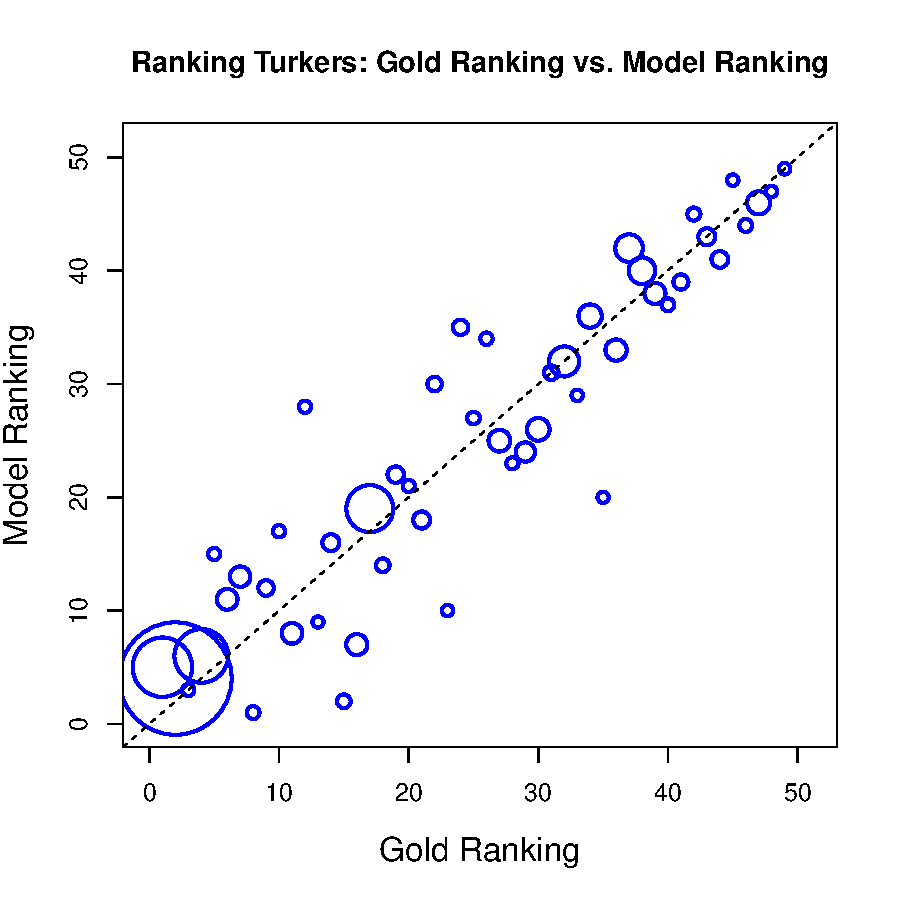
\includegraphics[width=\linewidth]{AllFeatureWithCali/allfeaturelinear.pdf}
  \caption{ Correlation between gold standard ranking and model ranking. %We train a linear regression model to score translations and to rank workers. 
The corresponding weighted correlation is 0.95. Each bubble represents a worker with his/her rank in gold standard ranking on x-axis and model ranking on y-axis. The radius of each bubble shows the relative volume of translations completed by the worker.}
    \label{modelrank}
\end{figure}
Figure \ref{modelrank} shows the high correlation between gold ranking and model ranking if all features are used in model tuning. Workers with high volumes of submissions are ranked extremely well.

\begin{table}[htbp]
 \center
\begin{tabular}{c|c|cc}
\hline
Feature Set             & $\rho$  & $B_r$ & $B_m$    \\ \hhline{====}
(S)entence features     & 0.84 & 36.66 &37.84 \\
(W)orker features       & 0.80 & 36.92 &36.92 \\
(R)anking features      & 0.81 & 36.94 &35.69\\
Calibration features  & 0.93 & 38.27 &38.27\\
%Calibration features* & \textbf{0.68} & \textbf{37.22} \\
S+W+R features          & 0.88 & 37.39 & 38.69\\
S+W+R+Bilingual features        & 0.89 & 37.59 &39.23 \\
All features            & \textbf{0.95} & \textbf{38.37} & \textbf{39.80}\\ \hline
%All features*            & \textbf{0.71} & \textbf{37.52} \\ \hline
\end{tabular}
\caption{\label{lrresult} Spearman's correlation($\rho$) and translation quality of selecting best translations based on model-predicted workers' ranking ($B_r$) and model predicted translations' scores ($B_m$) for different feature sets. We don't filter out bad workers when selecting the best translation.}
\end{table}
To reduce costs, we only keep hiring top workers and select the best translations based on their ranking. As comparison, we select the best translation using gold ranking. Table \ref{modeltoprank} shows the comparisons when we vary the top percentage of workers we keep hiring and the corresponding average number of non-professional translations needed for each source sentence. Comparing with selecting translations based on gold ranking, we achieve a similar BLEU score with lost of 0.55 when we filter out 75\% worker in tail and we only need to solicit two translations for each source sentence on average.


\begin{table}[htbp]
\center
\begin{tabular}{c|ccccc}
\hline
Top(\%) &$B_{r}$& $B_{t}$ & $B_{gold}$ & $\Delta$ & \# of Trans\\\hhline{======}
25      &29.85& 38.53   & 39.08      & 0.55   & 1.95         \\
50      &29.80& 38.40   & 39.00      & 0.60   & 2.73         \\
75      &29.76& 38.37   & 38.98      & 0.61   & 3.48         \\
100     &29.83& 38.37   & 38.99      & 0.62   & 4.00         \\ \hline
\end{tabular}
\caption{\label{modeltoprank}The comparison between translation quality of selecting translations based on model ranking ($B_{t}$) and gold ranking ($B_{gold}$) when we keep hiring different percentages of top workers. $\Delta$ is the different between $B_{gold}$ and $B_t$. \# of Trans is the average number of non-professional translations needed for each source sentence. $B_r$ is the BLEU score for random selection.
}
\end{table} 

\subsubsection{Ranking workers using their first k translations}
 Without using any model, we rank workers using their first k translations and select best translations based on rankings of top workers. To evaluate this method, we calculate the weighted correlation for our rankings against gold ranking. 
 %we created several test sets.  Each test set excluded any item that was used to rank the workers, or which did not have any translations from the top 25\% of workers according to our predicted rankings.  We therefore have \emph{different test sets} for each value of k.  This makes the results slightly more difficult to analyze than in normal experiments, although the trends are still clear.
%Formally, we define the test set for first k sentences as $T_k$ and for each source sentence $s \in T_k$:
%\begin{align*}
%  \{ s \mid (C(s) \cap S_k = \emptyset)   \wedge (C(s) \cap S_w \neq \emptyset)    \}
%\end{align*}
%where $C(s)$ is the translating candidates set of the source sentence $s$, $S_k$ is the translation set consists of each worker's first k translations and $S_w$ is the translation set consists of translations provided by selected workers (some top ranking workers). 
\begin{table}[h]
\begin{tabular}{cc|c}
\hline
\multicolumn{2}{c|}{\begin{tabular}[c]{@{}c@{}}Proportion of \\ Calibration Data\end{tabular}} & \multirow{2}{*}{\begin{tabular}[c]{@{}c@{}}$\rho$\end{tabular}}\\ \cline{1-2}
% & \multirow{2}{*}{\begin{tabular}[c]{@{}c@{}}$\rho^{*}$\end{tabular}} \\ \cline{1-2}
First k sentences                                 & Percentage                                 &                                                                                                                                          \\ \hhline{===}
1                                                 & 0.7\%                                      & 0.32                                                                                                                           \\
2                                                 & 1.3\%                                      & 0.36                                                                                                                                  \\
3                                                 & 2.0\%                                      & 0.35                                                                                                                                     \\
4                                                 & 2.7\%                                      & 0.59                                                                                                                                   \\
5                                                 & 3.3\%                                      & 0.70                                                                                                                                    \\
6                                                 & 4.0\%                                      & 0.75                                                                                                                                 \\
7                                                 & 4.7\%                                      & 0.76                                                                                                                                    \\
8                                                 & 5.3\%                                      & 0.73                                                                                                                                    \\
9                                                 & 6.0\%                                      & 0.78                                                                                                                                  \\
10                                                & 6.6\%                                      & 0.78                                                                                                                                    \\
20                                                & 13.3\%                                     & 0.91                                                                                                                                   \\
30                                                & 19.9\%                                     & 0.95                                                                                                                                 \\
40                                                & 26.6\%                                     & 0.97                                                                                                                                 \\
50                                                & 33.2\%                                     & 0.98                                                                                                                                   \\ 
60                                                & 39.8\%                                     & 0.99                                                                                                                                    \\ \hline
\end{tabular}
\caption{\label{spearmansen} Spearman's Correlations for calibration data in different proportion. 
%* indicates that the calibration is computed against \textbf{only one} reference while + indicates that the calibration is computed against 4 references.
}
\end{table}
Table \ref{spearmansen} shows the results of Spearman's correlations for different value of $k$. As $k$ increases, our rankings fit to the gold ranking better. Consequently, we can decide whether to continue to hire a worker in a very short time after analyzing the first k sentences ($k\le20$) provided by each worker. Figure \ref{first2hitrank} shows the correlation of gold ranking and first 20 sentences ranking. Since the weighted correlation score is 0.91, which means first 20 sentences ranking matches gold ranking well, we vary the top worker threshold on the first 20 sentences ranking and select translations by top workers ranking each time and calculate the BLEU score. 
\begin{figure}[h!]
  \centering
  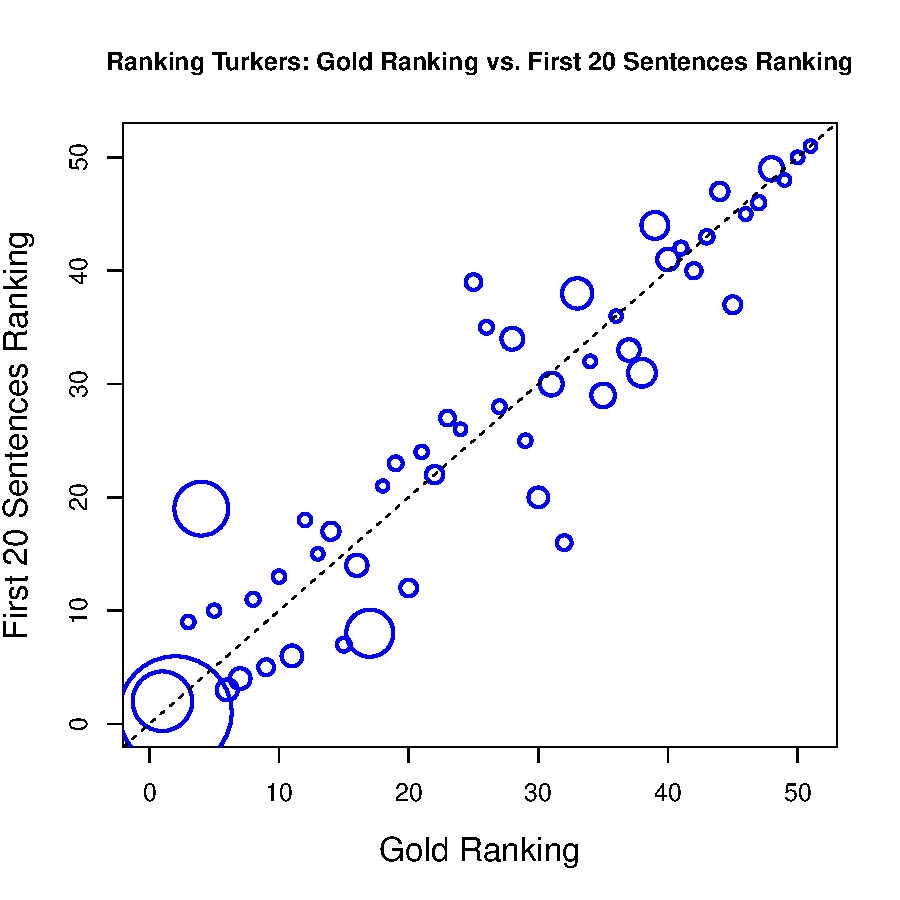
\includegraphics[width=\linewidth]{AllFeatureWithCali/2hitranking.pdf}
  \caption{ Correlation between gold standard ranking and first 20 sentences ranking. %We train a linear regression model to score translations and to rank workers. 
The corresponding weighted correlation is 0.91.
% Each bubble represents a worker with his/her rank in gold standard ranking on x-axis and model ranking on y-axis. The radius of each bubble shows the relative volume of translations completed by the worker.
}
    \label{first2hitrank}
\end{figure}
Table \ref{first20toprank} shows similar results as Table \ref{modeltoprank}. We can achieve a translation quality close to that of gold ranking selection with only soliciting half of non-professional translations if we keep hiring top 25\% workers after seeing 20 translations submitted from each of them.
\begin{table}[h!]
\center
\begin{tabular}{c|ccccc}
\hline
Top(\%) &$B_{r}$& $B_{t}$ & $B_{gold}$ & $\Delta$ & \# of Trans\\\hhline{======}
25      &28.76& 36.97   & 37.10      & 0.13   & 2.03         \\
50      &29.27& 36.90   & 37.15      & 0.25   & 2.60         \\
75      &28.89& 36.77   & 37.06      & 0.29   & 3.47         \\
100     &27.51&   36.77 & 37.06      & 0.29   & 4.00         \\ \hline
\end{tabular}
\caption{\label{first20toprank}The comparison between translation quality of selecting translations based on first 20 sentences ranking ($B_{t}$) and gold ranking ($B_{gold}$) when we keep hiring different percentages of top workers. $\Delta$ is the different between $B_{gold}$ and $B_t$. \# of Trans is the average number of non-professional translations needed for each source sentence. $B_r$ is the BLEU score for random selection.
}
\end{table} 

%Figure \ref{firstksenbleu}  shows the BLEU score when we select the top 25\% workers from the ranking list based on the performance of first k sentences.
%  As a comparison, we also plotted the  BLEU scores for random selection 
%  and the BLEU score for selection based on the gold standard ranking($B_{gold}$).
% %Figure \ref{firstksenbleudiff}  shows the difference between BLEU scores we get in three different mechanisms in order to make the comparisons clear.
%  As we increase the number of sentences we use to rank Turkers, the BLEU score we get from the ranking approaches $B_{gold}$. Surprisingly, we see that when only a small part of sentences (say 20 sentences) for each worker are used in ranking, the ranking list  is quite similar to the gold standard ranking list and the BLEU score is very close to the BLEU score get by gold standard ranking.
%\begin{figure}[h!]
%  \centering
%  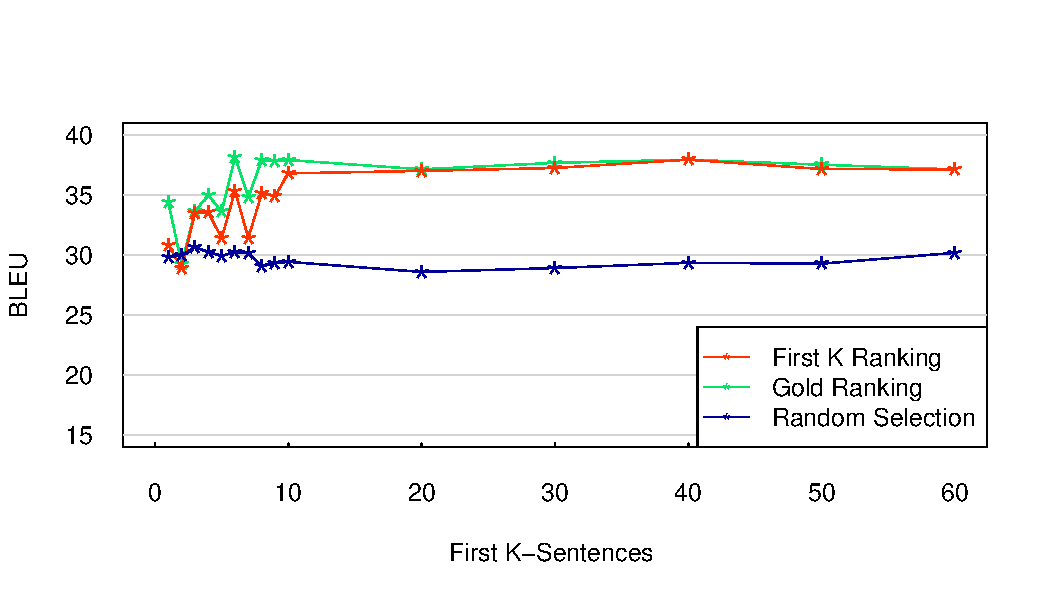
\includegraphics[width=\linewidth]{senlevelselect/curve1.pdf}
%  \caption{ The BLEU score for selecting the  best translation by the top 25\% Turkers' ranking based on the first k sentences (red line). The green line shows the BLEU score for selecting the best translation by the gold standard ranking. The dark blue line shows the BLEU score for selecting translation randomly.}
%    \label{firstksenbleu}
%\end{figure}
%
%\begin{figure}[h!]
%  \centering
%  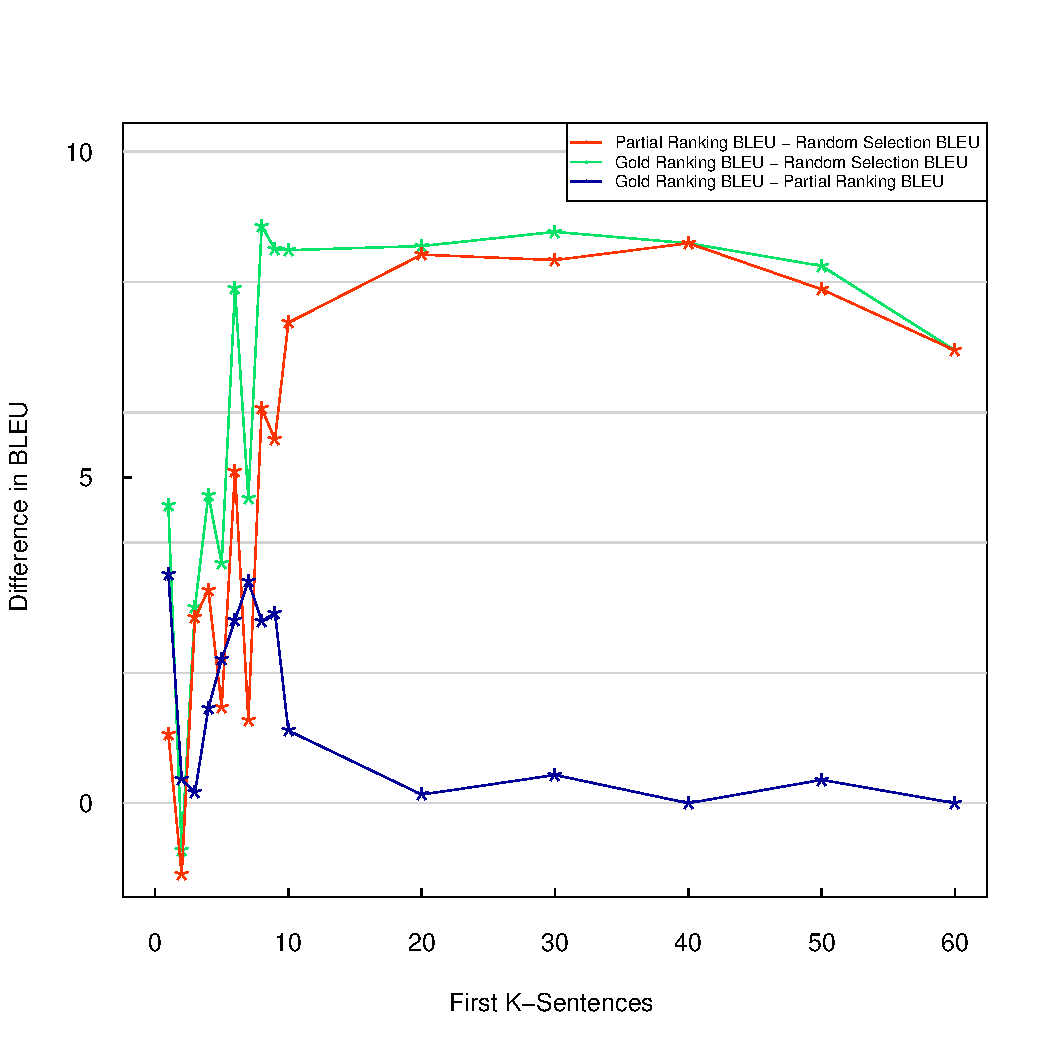
\includegraphics[width=\linewidth]{senlevelselect/curve2.pdf}
%  \caption{ The difference between BLEU scores reported from three different methods in Figure \ref{firstksenbleu}.}
%   \label{firstksenbleudiff}
%  \end{figure}

%If we use the first 20 sentences to rank workers, the correlation is 0.88 and  the BLEU score achieved is 37.01 while  and $B_{gold}$ is 37.14. The difference between these two scores is 0.13 and the cost is: \\
%  \begin{align*}
%  C& = \frac{\alpha}{4} \cdot  (0.133 \cdot N_{p}) \cdot C_{p}  + \frac{\beta }{4}\cdot (0.867\cdot N_{np} ) \cdot C_{np}\\
%   & = 1,592.53 (\$)
%  \end{align*}  
%We can achieve almost the same translation as the oracle method with only spending 32\% of the total cost. 


\section{Cost Analysis}

 We have introduced several ways of significantly lowering the costs associated with crowdsourcing translations when a large amount of data are solicited (on the order of millions of samples):
\begin{itemize}
\item We show that after we have collected one translation of a source sentence, we can consult a model that predicts whether its quality is sufficiently high or whether we should pay to have the sentence re-translated.  The cost savings for non-professionals here comes from reducing the number of redundant translations. We can save half of the cost associated with non-professional translations to get 95\% of the translation quality using the full set of redundant translations.
\item We show that we can quickly identify bad translators, either with a model designed to rank them, or by ranking them by having them first translate a small number of sentences with gold standard translations. The cost savings for non-professionals here comes from not hiring bad workers. Similarly, we reduce the non-professional translation cost to the half of the original cost.

\item In both cases we need a some amount of professionally translated materials  to use as a gold standard for calibration. Although the unit cost for each reference is much higher than the unit cost for each non-professional translation, the cost associated with non-professional translations can dominate the total cost since the large amount of data need to be collected. Thus, we focus on reducing cost associated with non-professional translations. 
%The cost savings for professionals come from reducing the referencing translations to calibrate each data sample. 
% The cost of these professional translations can dominate the cost of our models, so we experiment with how little we can get away with.
\end{itemize}
%In all cases, there is a trade-off between lowering our costs and producing high quality translations.  Figure \ref{fbleucost} plots the cost versus the BLEU scores for the different configurations that we experimented with.
%
%In Figure \ref{fbleucost}-(a) the increasing costs are a function of how many sentences we use to rank the translators.  Here we use no model, and simply rank the translators by their BLEU score against a small amount of gold standard data. The quality peaks at 37.9 BLEU after \$3,000.
%%the return on investment is low after spending the first \$2,000 to get a BLEU of 35.6.
%We are able to rank the translators with high accuracy and achieve a relative high BLEU score by paying for a comparatively small number of professional translations to use as calibration. From our experiments,  10-20 professionally translated sentences seems like a reasonable number. 
%
%Figure\ref{fbleucost}-(b) uses a model to determine whether to purchase another translation.  
%%Here the starting cost is high (nearly \$9,000) because the model requires a significant amount of professional translations in order to train the model and to determine the optimal threshold values for whether to solicit another translation. 
%This model allows us to significantly improve the overall translation quality to a BLEU score of nearly 40, for a final cost of \$2,700.
%
%%To emphasize the effectiveness of model selection approach, Figure \ref{fbleucost}-(c) plots the relationship between BLEU and non-professional component of the overall cost.  Past approaches to crowdsourcing translation always solicited 4 non-professional translations of every source sentence. The cost for translating our 1433 test sentences under this approach is \$573.44.  This produces the maximum BLEU score of 40.1.  Using our model to reduce the number of redundant translations, we can reduce the costs with mild degredation in translation quality.  We can cut the number of non-translations in half, and pay only \$286.72, while achieving a BLEU score of 37.6 (94\% of the maximum), or pay \$348.36,60.7\% of total non-professional translations' cost, for a BLEU of 38.5 (96\% of  the maximum).
%
%\begin{figure}[htbp]
%  \centering
%  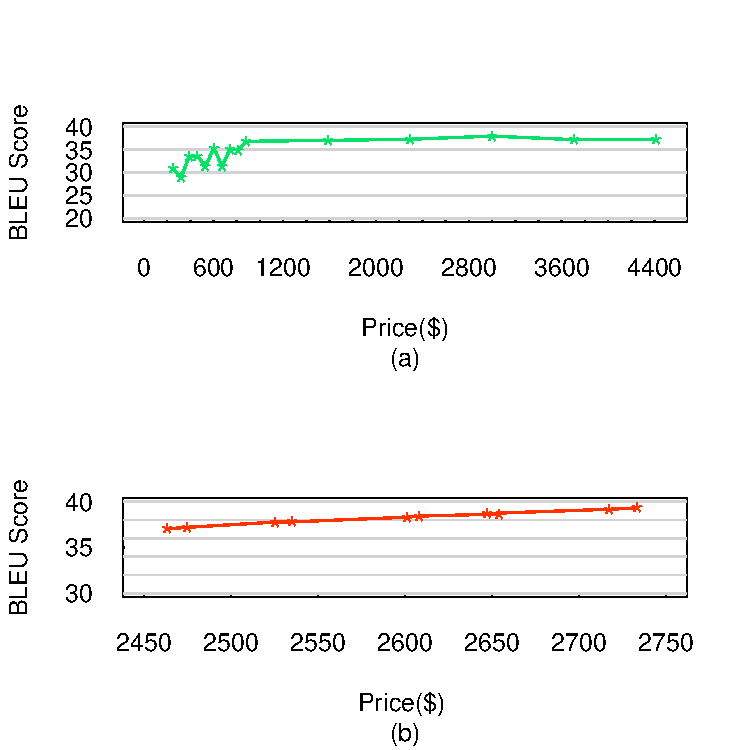
\includegraphics[width=\linewidth]{cost-bleu/pricecost.pdf}
%  \caption{The Relationship between BLEU score and costs. In Figure (a), the red line shows the relationship between BLEU score and  the total costs (professional and non-professional) for the ranking based approach. 
%  %The green line shows the corresponding translation quality for gold standard ranking selection measured in BLEU score. 
%  Figure (b) shows the relationship between BLEU score and the total costs for model-based approach. 
%  %Figure (c)  illustrates the relationship between BLEU score and non-professional costs for model based approach.
%  }
%    \label{fbleucost}
%\end{figure}
\section{Related Work}
%Crowdsoucing has been widely used in data annotation or labeling to get a large amount of data at low cost. The relationship between the budget and the quality was discussed in previous work.

\newcite{sheng2008get}'s work on repeated labeling presents a way of solving the problems of uncertainty in labeling. Since we cannot always get high-quality labeled data samples with relatively low costs in reality, to keep the model trained on noisy labeled data having a high accuracy in predicting, \newcite{sheng2008get} proposed a framework for repeated-labeling that resolves the uncertainty in labeling via majority voting. The experimental results show that a model's predicting accuracy is improved even if labels in its training data are nosity and of imperfect quality.  As long as the integrated quality (the probability of the integrated labeling being correct) is higher than 0.5, repeated labeling benefits model training. 

\newcite{passonneau2013benefits} created a Bayesian model of annotation and they applied to the problem of word sense annotation. \newcite{passonneau2013benefits} also proposed an approach to detect and avoid spam workers. 
%They required workers to finish 20000 HITs and have a 98\% lifetime approval rating. 
They measured the performance of worker by comparing worker's labels to the current majority labels and worker with bad performance would be blocked. However, this approach suffered from 2 shortcomings: (1) Sometimes majority labels may not reflect the ground truth label. (2) They didn't figure out  how much data(HITs) is needed to evaluate a worker's performance. Although they could find the spam after the fact, it was a post-hoc analysis, so they had already paid for that worker and wasted the money.

\newcite{lin2014re} examined the relationship between worker accuracy and budget in the context of using crowdsourcing to train a machine learning classifier.  They show that if the goal is to train a classifier on the labels, that the properties of the classifier will determine whether it is better to re-label data (resulting in higher quality labels) or get more single labeled items (of lower quality). They showed that classifiers with weak inductive bias  benefit more from relabeling, and that relabeling is more important when worker accuracy is low (barely higher than 0.5). 

\newcite{novotney2010cheap} showed a similar result for training an automatic speech recognition (ASR) system.  When creating training data for an ASR system, given a fixed budget. Their system's accuracy was higher when it is trained on more low quality transcription data compared to when it was trained on fewer high quality transcriptions.


\section{Conclusion}
In this paper, we propose two mechanisms to optimize cost: the translation reducing method and the translator reducing method. They have different applicable scenarios for large corpus construction.
The translation reducing method works if there exists a specific requirement that the quality control must reach a certain threshold. 
This model is most effective when reasonable amounts of pre-existing professional translations are available for setting the models threshold. 
 %Its major cost reduction comes from dramatically reducing the amount of non-professional data to maintain the high quality.
The translator reducing method is very simple and easy to implement. This approach is inspired by the intuition that workers' performance is consistent. The translator reducing method is suitable for crowdsourcing tasks which do not have specific requirements about the quality of the translations, 
%or when the data collection is being performed by a requester who does not have sufficient background in machine learning in order to train a model, 
or when only very limited amounts of gold standard data are available.


 

%We kept the `best' translators, defining the best as the top 25\% workers in our ranked list.  The idea is to retain only the top-performing workers, and to make that decision quickly (after seeing only k of their translations).  

%\subsection{Comparability of Translation Quality between Different Translation Selection Strategies}
%To show the comparability of translation quality between ranking selection strategy and model selection strategy, we train MERT, Regression Trees, and Linear Regression models to rank translators, calculate rankings' correlations against the gold standard ranking and compare the translation qualities between ranking selection and model selection. Besides features \cite{Zaidan09zmert} used, we introduce a new bilingual feature. We use the IBM Model 1 to construct the word alignment with probabilities between Urdu and English. For each foreign sentence, we calculate the word alignment feature by averaging the alignment probabilities of all words in Urdu sentence. 
% We evaluate models through five-fold cross validation. We divided the data into 2 parts: 20\% data for feature values calculations and remaining 80\% data for testing. We use the  20\% portion to calculate the worker aggregation feature, and half of the data in the 20\% portion (10\% of the full data set ) to calculate the worker calibration feature against their references.  This 10\% portion of data is used as training set where the label of each sample is the BLEU score against 4 references. %Since we want to show that we can save money by reducing professionals translation as calibration, the proportion of the training set is smaller than that in general machine learning problem. 
%We use the training data to create a model, which we denote as $M$. For each source sentence $s_i$, we have a translation set $T = \{ t_{i,1}, t_{i,2},t_{i,3}, t_{i,4}\}$. %We select the translation with highest model predicted score $M(t)$.
%The model predicted score for translation $t$ is defined as $M(t)$.
%%For MERT and Linear Regression, $M$ is a vector of weights  corresponding to  dimensions in the feature space. $M(t)$ is defined as:
%% \begin{align*}
%%  M(t) = \hat{w}  \cdot f(t) 
%%  \end{align*}
%%  where $\hat{w}$ is weight vector and $f(t)$ is the feature vector of the translation $t$. For Regression Tree, $M$ is a tree where each internal node has a threshold to split on the corresponding dimension and each leaf node has the BLEU score value. 
%%  
%Using the remaining 80\% of the data as our test set, first we rank workers by their performance predicted by models and evaluate the ranking list by calculating the Spearman's correlation against the gold standard ranking. The performance of the worker $w$ according to a model is computed as:
%\begin{align*}
%Performance(w) = \frac{\sum_{t \in T_{w}} M (t)}{|T_{w}|}
% \end{align*}
% where $T_{w} $ is the set of translations completed by $w$. 
%%  \begin{table}[t]
%% %\begin{center}
%% \center
%% \begin{tabular}{|c|c|c|c|}
%%\hline
%%\multirow{2}{*}{Feature Set} & \multicolumn{3}{c|}{Spearman Correlation}                                                                 \\ \cline{2-4} 
%%                             & \multicolumn{1}{l|}{MERT} & \multicolumn{1}{l|}{LR\tablefootnote[2]{\label{note2}Linear Regression} } & \multicolumn{1}{l|}{RT\tablefootnote[3]{ \label{note3}Regression Tree}  } \\ \hline
%%Sentence features            & 0.36                      & 0.69                                   & 0.71                                 \\ \hline
%%Worker features              & 0.44                      & 0.65                                   & 0.59                                 \\ \hline
%%Ranking features             & 0.67                      & 0.79                                   & 0.76                                 \\ \hline
%%Calibration feature          & 0.79                      & 0.79                                   & 0.79                                 \\ \hline
%%S+W+R features  \tablefootnote[4]{\label{note4}Combination of (S)entence, (W)orker and (R)anking features}            & 0.42                      & 0.78                                   & 0.74                                  \\ \hline
%%S+W+R+B features   \tablefootnote[5]{\label{note5}Combination of (S)entence, (W)orker , (R)anking and (B)ilingual features}           & 0.47                      & 0.80                                   & 0.72                                 \\ \hline
%%All features                 & 0.56                      & 0.84                                   & 0.81                                 \\ \hline
%%\end{tabular}
%% %\end{center}
%% \caption{\label{spearmanrho} Spearman's correlation for different models trained using different feature sets }
%%\end{table}
%%
%%\begin{table*}[t]
%%\begin{center}
%%
%%\begin{tabular}{|c|c|c|c|c|c|c|}
%%\hline
%%\multirow{2}{*}{Feature Set} & \multicolumn{3}{c|}{Bleu Score (selected by ranking)} & \multicolumn{3}{c|}{Bleu Score (selected by model)} \\ \cline{2-7} 
%% & MERT      & LR \footnotemark[\ref{note2}]    & RT \footnotemark[\ref{note3}]    & MERT     & LR  \footnotemark[\ref{note2}]   & RT \footnotemark[\ref{note3}]     \\ \hline
%%Sentence features            & 30.04     & 36.66                & 36.97              & 38.51    & 37.84                & 35.32             \\ \hline
%%Worker features              & 37.89     & 36.92                & 37.96              & 37.89    & 36.92                & 37.59             \\ \hline
%%Ranking features             & 37.25     & 36.94                & 37.04              & 36.74    & 35.69                & 36.17             \\ \hline
%%Calibration feature          & 38.27     & 38.27                & 38.27              & 38.27    & 38.27                & 38.27             \\ \hline
%%S+W+R features\footnotemark[\ref{note4}]              & 33.04     & 37.39                & 37.60              & 38.44    & 38.69                & 37.04             \\ \hline
%%S+W+R+B features  \footnotemark[\ref{note5}]           & 34.30     & 37.59                & 37.27              & 38.80    & 39.23                & 37.00             \\ \hline
%%All features                 & 35.58     & \textbf{38.37}                & \textbf{37.80}              & 39.74    & \textbf{39.80}                & \textbf{37.19}             \\ \hline
%%\end{tabular}
%%\end{center}
%%\caption{\label{bleu} Bleu score for different models trained using different feature sets }
%%\end{table*}
%
%For each test sample, we select the translation  provided by the worker with the best rank, and evaluate the translation quality by calculating the BLEU score against references.  As a comparison, for the same test sample, we also select the translation with the highest  model predicted score and evaluate translation quality. Table \ref{spearmanrho} presents ranking lists' correlation scores corresponding to different models trained using different features.  Table \ref{bleu} shows the translation quality comparisons for the two selecting strategies. From Table \ref{spearmanrho} and  Table \ref{bleu}, we know that if the predicted ranking list is highly correlated to the gold standard ranking, the translation quality of ranking selection method is comparable to that of model selection method. Besides, as a comparison, if we directly compute the gold standard ranking of all translators using all of the data and select translation based on the gold ranking, then the BLEU score ($S_{rgold}$) is 38.99, which is quite close to 39.80 ($S_{mgold}$), the highest BLEU score we get by model selection method. Thus, it's reasonable to use  $S_{rgold}$ as the upper-bound of the translation quality instead of $S_{mgold}$ since it's difficult to compare translation qualities between a ranking selection method and a model selection method on dynamic testing sets. Table \ref{spearmanrho} shows an unexpected result. The MERT trained on the complete set of features produces a correlation that is weaker than one trained only use ranking features.  The reason for this is that the model is trained using the MERT algorithm \cite{och2003minimum}, which is typically used to set the parameters of a statistical machine translation system such that the 1-best translation is ranked the highest among an $n$-best list containing thousands of translations. Setting the feature weights using MERT does a poor job at producing a total ordering on the translators. 
%
%\subsection{Baselines}
%We set two baselines for ranking correlation for our proposed approaches. For the first baseline,  we choose the MERT baseline, which achieves a correlation of  0.67 when trained on ranking features. This is the highest correlation that  MERT achieves across all feature sets. The second baseline is a simpler baseline that reserves 10\% of the data for calibration, and computes a ranking of translators based on their BLEU scores against the professionals over this calibration set, the correlation reaches 0.79.  
% 
% \subsection{Save Cost by Filtering out Bad Workers}
% \subsubsection{Ranking workers using a model}
%Table \ref{bleu} shows that the Logistic Regression Model achieves the highest BLEU score trained on all features among all ranking selection methods. Thus we train a Logistic Regression Model to rank workers and keep retaining top 25\% workers. 
%%In each test sample in the testing set,there exists at least one translation provided by the worker among the top 25\%. 
%In testing, we only select the translation with the best rank provided by top workers. We achieve a high ranking correlation of 0.84 and a BLEU score of 37.94 while $S_{rgold}$ is 38.99. The difference between these two BLEU scores is 1.05. The cost is:
% \begin{align*}
%  C& = 10\% \cdot N_{p}\cdot C_{p}  + (1-10\% )\cdot 25\% \cdot N_{np} \cdot C_{np}\\
%   & = 0.1 \cdot N_{p}\cdot C_{p}  + 0.225\cdot N_{np} \cdot C_{np}
%  \end{align*}
% \subsubsection{Decide whether hire workers after their first $k$ translations}
%Rather than using a model to rank workers, we use the quality of first-K translation sentences provided by each Turker as calibration to rank workers. The translation quality is computed against references. Table \ref{spearmansen} shows the results of Spearman's Correlation for different value of K.  We get a surprisingly strong correlation with the gold standard ranking of workers, without using a model at all. 
%We achieve  very strong correlation when calibrating the workers based on  the translations of their first 40 sentences. Even we only use the first 10 sentences to evaluate and rank workers, the correlation ($\rho$) is higher than 0.80. If we use the first 20 sentences, which is still only a small  part of data compared with the whole data set, $\rho$ is higher than 0.90, nearly a perfect match with the gold standard ranking. Consequently, we can decide whether to continue to hire a worker in a very short time after analyzing the first k sentences (k may be equal to or less than 10) provided by each worker. 
%We kept the `best' translators, defining the best as the top 25\% workers in our ranked list.  The idea is to retain only the top-performing workers, and to make that decision quickly (after seeing only k of their translations).  
%
%\begin{figure}[h!]
%  \centering
%  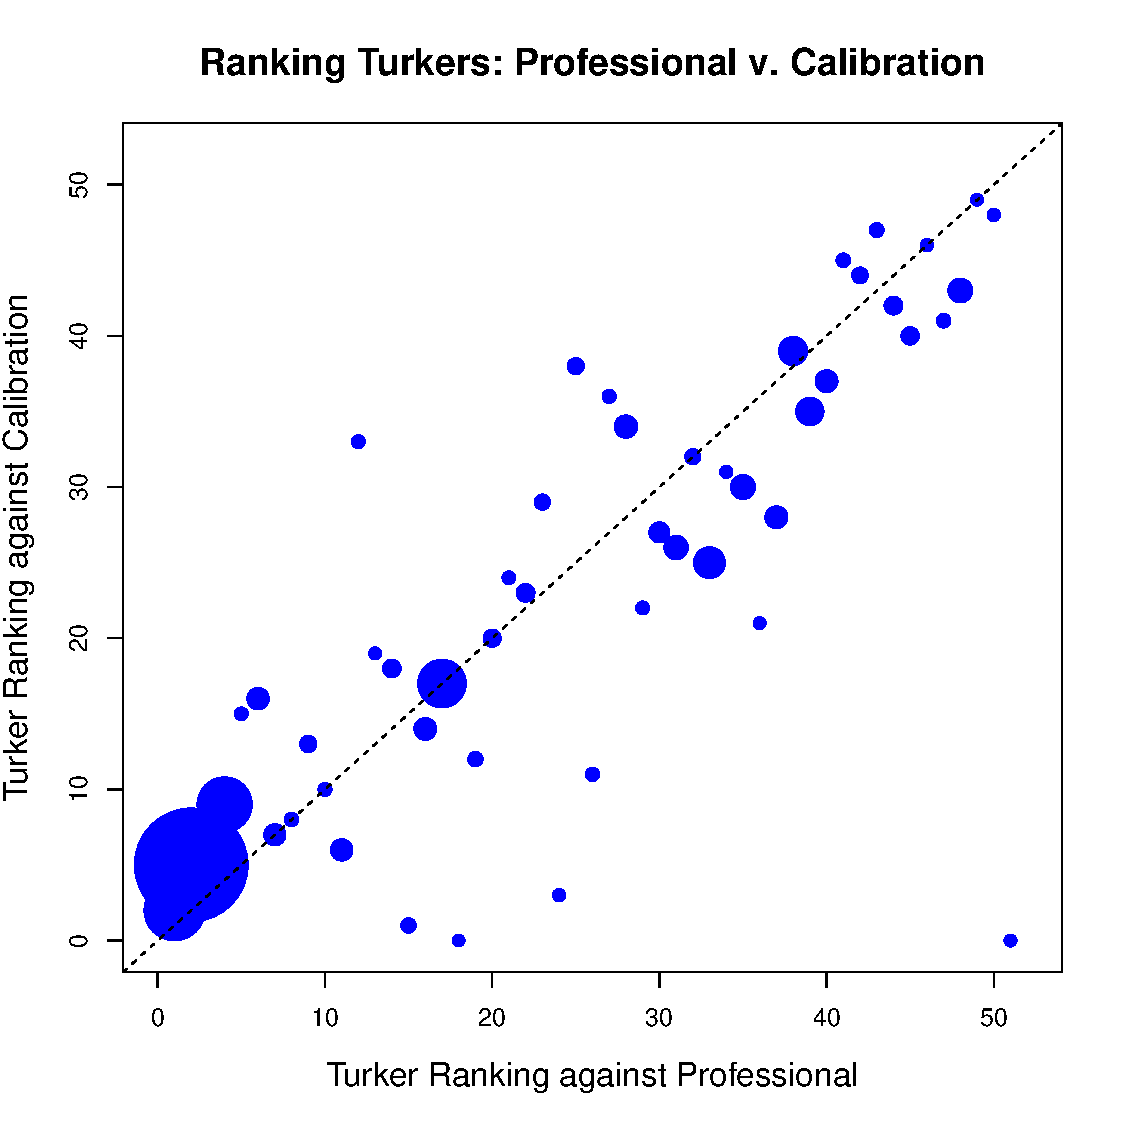
\includegraphics[width=\linewidth]{OnlyCali/calirankingorder.pdf}
%  \caption{Correlation between gold standard ranking and calibration ranking. We use 10\% training data as calibration data to rank workers. The corresponding Spearman's Correlation is 0.79. Each bubble represents a worker with his/her rank in gold standard ranking on x-axis and rank in calibration ranking on y-axis. The radius of each bubble shows the relative volume of translations completed by the worker.  }
%    \label{fdtallwocalbutbilinorder}
%\end{figure}
%
%
%\begin{table}[h]
%\begin{center}
%\begin{tabular}{|c|c|c|}
%\hline
%\multicolumn{2}{|c|}{\begin{tabular}[c]{@{}c@{}}Proportion of \\ Calibration Data\end{tabular}} & \multirow{2}{*}{\begin{tabular}[c]{@{}c@{}}Spearman's \\ Correlation\end{tabular}} \\ \cline{1-2}
%First k Sentence                                     & Percentage                                    &                                                                                    \\ \hline
%1                                              & 0.7\%                                         & 0.57
% \\ \hline
%2                                              & 1.3\%                                         & 0.62
% \\ \hline
%3                                              & 2.0\%                                         & 0.69
% \\ \hline
%4                                              & 2.7\%                                         & 0.72
% \\ \hline
%5                                              & 3.3\%                                         & 0.78
% \\ \hline
%6                                              & 4.0\%                                         & 0.80
% \\ \hline
%7                                              & 4.7\%                                         & 0.79
% \\ \hline
%8                                              & 5.3\%                                         & 0.81
% \\ \hline
%9                                              & 6.0\%                                         & 0.84
% \\ \hline
%10                                               & 6.6\%                                         & 0.84                                                                              \\ \hline
%20                                              & 13.3\%                                        & 0.93                                                                               \\ \hline
%30                                               & 19.9\%                                        & 0.96                                                                               \\ \hline
%40                                               & 26.6\%                                        & 0.97                                                                               \\ \hline
%50                                               & 33.2\%                                        & 0.98                                                                               \\ \hline
%60                                               & 39.8\%                                        & 0.99                                                                               \\ \hline
%70                                               & 46.5\%                                        & 0.99                                                                               \\ \hline
%80                                               & 53.1\%                                        & 0.99                                                                               \\ \hline
%90                                               & 60.0\%                                        & 0.99                                                                               \\ \hline
%100                                              & 66.4\%                                        & 0.99                                                                               \\ \hline
%\end{tabular}
%\end{center}
%\caption{\label{spearmansen} Spearman's Correlation for calibration data in different proportion}
%\end{table}
%To evaluate this method, we created several test sets.  Each test set excluded any item that was used to rank the workers, or which did not have any translations from the top 25\% of workers according to our predicted rankings.  We therefore have \emph{different test sets} for each value of k.  This makes the results slightly more difficult to analyze than in normal experiments, although the trends are still clear.
%
%Formally, we define the test set for first k sentences as $T_k$ and for each source sentence $t \in T$:
%\begin{align*}
%  \{ t \mid (C(t) \cap S_k = \emptyset)   \wedge (C(t) \cap S_w \neq \emptyset)    \}
%\end{align*}
%where $C(t)$ is the translating candidates set of the source sentence t, $S_k$ is the translation set consists of each worker's first k translations and $S_w$ is the translation set consists of translations provided by selected workers (some top ranking workers).
%
%\begin{figure}[h!]
%  \centering
%  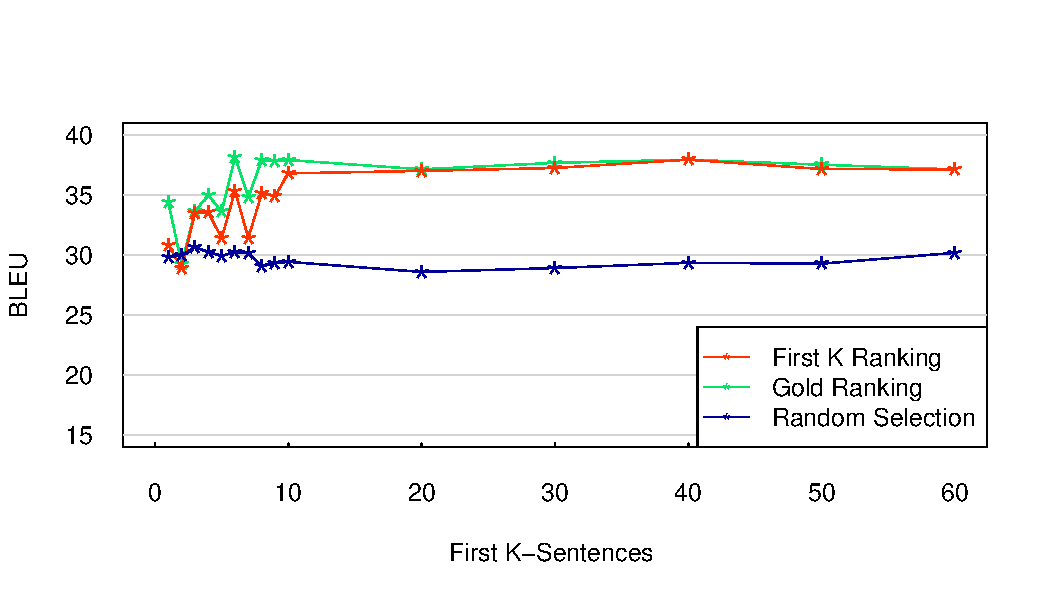
\includegraphics[width=\linewidth]{senlevelselect/curve1.pdf}
%  \caption{ The BLEU score for selecting the  best translation by the top 25\% Turkers' ranking based on the first k sentences (red line), which is denoted as Partial Ranking BLEU. The green line shows the BLEU score for selecting the best translation by the gold standard ranking, which is denoted as Gold Ranking BLEU. The dark blue line shows the BLEU score for selecting translation randomly. We denote it as Random Selection BLEU.}
%    \label{firstksenbleu}
%\end{figure}
%\begin{figure}[h!]
%  \centering
%  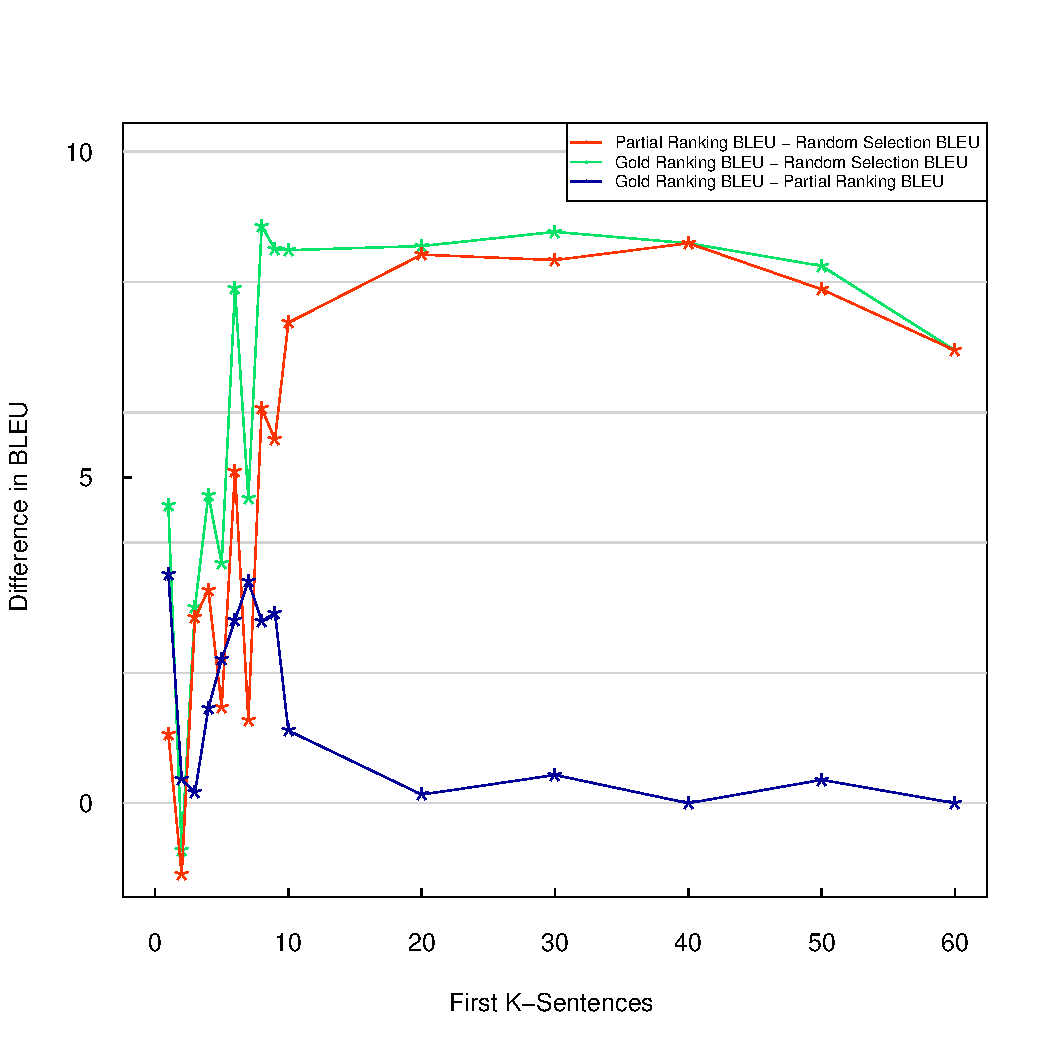
\includegraphics[width=\linewidth]{senlevelselect/curve2.pdf}
%  \caption{ The difference between BLEU scores reported from three different methods in Figure \ref{firstksenbleu}.
%%The green line shows the difference between  Gold Ranking BLEU and Random Selection BLEU.  The red lines shows the difference between Partial Ranking BLEU and Random Selection BLEU and the dark bleu line shows the difference between methods Gold Ranking BLEU and Partial Ranking BLEU.
%}
%    \label{firstksenbleudiff}
%\end{figure}
%
%%In the first approach, we quickly evaluate workers and rank them for filtering out workers with low rankings. We train linear regression models using a variety of features to score each translation and evaluate workers by averaging the scores of his/her translations. 
%
%
%%Table \ref{spearmanrho} shows that the higest correlation is achieved using the Linear Regression model trained on all features, including the sentence, worker, ranking, bilingual and calibration features.  It achieves a Spearman's Correlation of 0.84.  Since we  use 10\% data to calculate calibration feature, and since professional translators are used to created the calibration data, its cost is approximately \$ XXX (XXX * YYY sentences or words). 
%
%%The Linear Regression model with all features acheives a BLEU score of 38.37, its ranked list of translators  is used ot select the best translation for each source sentence.  The difference between these two BLEU scores is 0.62. We save 90\% cost for LDC data with the penalty of losing 0.62 BLEU score in selecting accuracy.
%
%  
%  Figure \ref{firstksenbleu}  shows the BLEU score when we select the top 25\% workers from the ranking list based on the performance of first k sentences.
%  %, which is denoted as $B_{k}$.  
%  As a comparison, we also plotted the  BLEU scores for random selection 
%%  ($B_{r}$) 
%  and the BLEU score for selection based on the gold standard ranking.
% %  ($B_{g}$).  
% Figure \ref{firstksenbleudiff}  shows the difference between BLEU scores we get in three different mechanisms in order to make the comparisons clear.
%  As we increase the number of sentences we use to rank Turkers, the BLEU score we get from the ranking approaches the BLEU score ($B_{g}$) we get by selecting translations based on the gold standard ranking. Surprisingly, we see that when only a small part of sentences (say 10 sentences) for each worker are used in ranking, the ranking list  is quite similar to the gold standard ranking list and the BLEU score is very close to the BLEU score get by gold standard ranking.
%  
%  If we use the first 10 sentences,  the correlation is 0.84 and  $B_{10}$ is 35.77 and $B_{g}$ is 37.57. The difference between $B_{g}$ and $B_{10}$ is 1.8 while the cost is: \\
%  \begin{align*}
%  C& = 6.6\% \cdot N_{p}\cdot C_{p}  + (1-6.6\% )\cdot 25\% \cdot N_{np} \cdot C_{np}\\
%   & = 0.066 \cdot N_{p}\cdot C_{p}  + 0.2335 \cdot N_{np} \cdot C_{np}
%  \end{align*}
% which is only a small part of the whole cost. If we increase the number of sentences we use for ranking to 20, the correlation increase to 0.93 and $B_{20}$ is 36.97. The difference decreases to 0.13 and the cost is:
%\begin{align*}
%C& = 13.3\% \cdot N_{p}\cdot C_{p}  + (1-13.3\% )\cdot 25\% \cdot N_{np} \cdot C_{np}\\
%   & = 0.133 \cdot N_{p}\cdot C_{p}  + 0.21675 \cdot N_{np} \cdot C_{np}
%\end{align*}
%    
% \section{Get Another Translation?}
% % New Version
% 
%% In the second approach,  we train a model to decide whether a translation is 'good enough,' in which case we don't need to pay for another redundant  translation of the source sentence.  
%% % End
% 
% \begin{table}[h]
%\begin{tabular}{|c|c|c|c|}
%\hline
%
%\textit{delta} (\%) & $S_{upper}$ & BLEU Score & \textit{\# of Trans} \\ \hline
%90         & 40.13       & 36.46      & 1.67       \\ \hline
%91         & 40.13       & 36.72      & 1.75       \\ \hline
%92         & 40.13       & 36.84      & 1.77       \\ \hline
%93         & 40.13       & 37.11      & 1.87       \\ \hline
%94         & 40.13       & 37.61      & 2.00       \\ \hline
%95         & 40.13       & 37.90      & 2.12       \\ \hline
%96         & 40.13       & 38.32      & 2.31       \\ \hline
%97         & 40.13       & 38.52      & 2.43       \\ \hline
%98         & 40.13       & 39.12      & 2.79       \\ \hline
%99         & 40.13       & 39.45      & 3.05       \\ \hline
%100        & 40.13       & 39.90      & 3.58       \\ \hline
%\end{tabular}
%\caption{The relation among the \textit{delta} (the proportion of the BLEU score's upper bound $S_{upper}$),the BLEU score for translations selected by models and the averaged size of translation candidates set for each source sentence (\textit{\# of Trans}).  }
%    \label{orderanother}
%\end{table}
%We present the model selection method to decide whether a translation  is `good enough,' in which case we don't need to  pay for another redundant translation of the source sentence. Besides, we quantify the quality control  issue: make it possible to control the BLEU score of the translation selected from a partial translation set to a proportion (\textit{delta}) of the upper bound of BLEU score. The upper bound of BLEU score is computed on best translations selected from  the full translation set. For a specific delta value, we train the Linear Regression model to score each translation we've got already, and use this score comparing with the threshold between acceptable and unacceptable translations to evaluate whether to get another translation. If the translation's 
%% we solicit currently satisfies our quality control demand which means the 
% model predicted BLEU score is higher than the threshold, we stop soliciting other translations continually for the source sentence. Table \ref{texample} illustrates the idea of this approach. On one hand, since we only collected part of the full translation candidates set, we save money by avoiding paying for  redundant   translations.  On the other hand, in the training and validating process, we reduce the size of the training set and validation set, say only 10\% of the full data set for each , which means we only need 10\% reference data to calculate the gold standard BLEU score and calibration feature value for each translation candidate in training set and validation set respectively. 
% 
% \begin{table*}[t]
% \center
%\begin{tabular}{|c|c|c|c|}
%\hline
%Source                                   & References                         & Translations                         & Quality \\ \hline
%\multirow{4}{*}{فرانس کی تجویز کی حمایت} & Support of France's Recommendation & France has supported the proposal.   & 0.342   \\ \cline{2-4} 
%                                         & Support for the Proposal of France & Supporting the French proposal       & 0.630   \\ \cline{2-4} 
%                                         & French Proposal Endorsed           & France suggestion was appriciatable. & -0.014  \\ \cline{2-4} 
%                                         & French Proposal Supported          & defending the thinking of France.    & 0.269   \\ \hline
%\end{tabular}
%\caption{An example showing how to reduce redundant translations using the  model and the threshold. For each source sentence, we solicit 4 references and 4 non-professional translations. The value of 'Quality' is the \textbf{ model predicted score} for each translation which is different from the BLEU score. In this example, \textit{delta} is \%95, and the threshold telling apart acceptable and unacceptable translations is 0.35. Translations listed from top to the bottom are in the chronological order from the earliest submitted one to the latest submitted one. Since the first translation's quality value is lower that the threshold, we need to solicit another one.  Knowing that the second translation's quality value is higher than the threshold,  we stop soliciting other translations for this source sentence so that we avoid collect redundant translations and reduce cost.}
%\label{texample}
%\end{table*}
% 
%To evaluate the performance of the model running with different thresholds, we first compute an upper bound by selecting the best translation among all 4 candidates for each foreign sentence of the validation set according to our  model. We call this  $S_{upper}$.  $S_{upper}$ is the highest BLEU score we can get by choosing translation using the model, since it has access to all of the available translations. Originally, for each source sentence, the size of the translation set is 4. Since we stop soliciting translations after getting the acceptable one, the averaged size of translation set among all source sentences becomes less than 4. We define the averaged size of translation sets as \textit{\# of trans}.
%
%Table \ref{orderanother} shows the  positive correlations between  \textit{delta} and \textit{\# of Trans}.
%%\begin{align*}
%%\textit{\# of Trans} \propto \textit{delta} 
%%\end{align*}
%Thus, it's reasonable to deduce the negative correlations between the cost and \textit{delta}.  From Table \ref{orderanother}, we see that as the  translating accuracy (\textit{delta} and BLEU score) increasing, the averaged size of translation set increases.  
% \subsection{Experimental Setup}
% In experiment, we divide the data into 3 parts: 10$\%$ of the data as a training set, 10$\%$ of the data as a validation set and the remaining 80$\%$ of the data as a test set. 
%
%After  training  a Linear Regression model, the challenge we are facing with is how to set the threshold to separate acceptable translations and unacceptable ones. 
% 
% 
%% Maybe first describe the model features, and then describe how you set the threshold value. 
% In our design, we set the threshold empirically using the validation set after we have trained the model on the disjoint training set. More specifically, during the training process, we get the upper bound of scores for translations in the training set. Then we search for the threshold through traversing from  zero to the upper bound by a small step size. %add a figure to illustrate the traversal
% 
%% \begin{figure}[htbp]
%%  \centering
%%  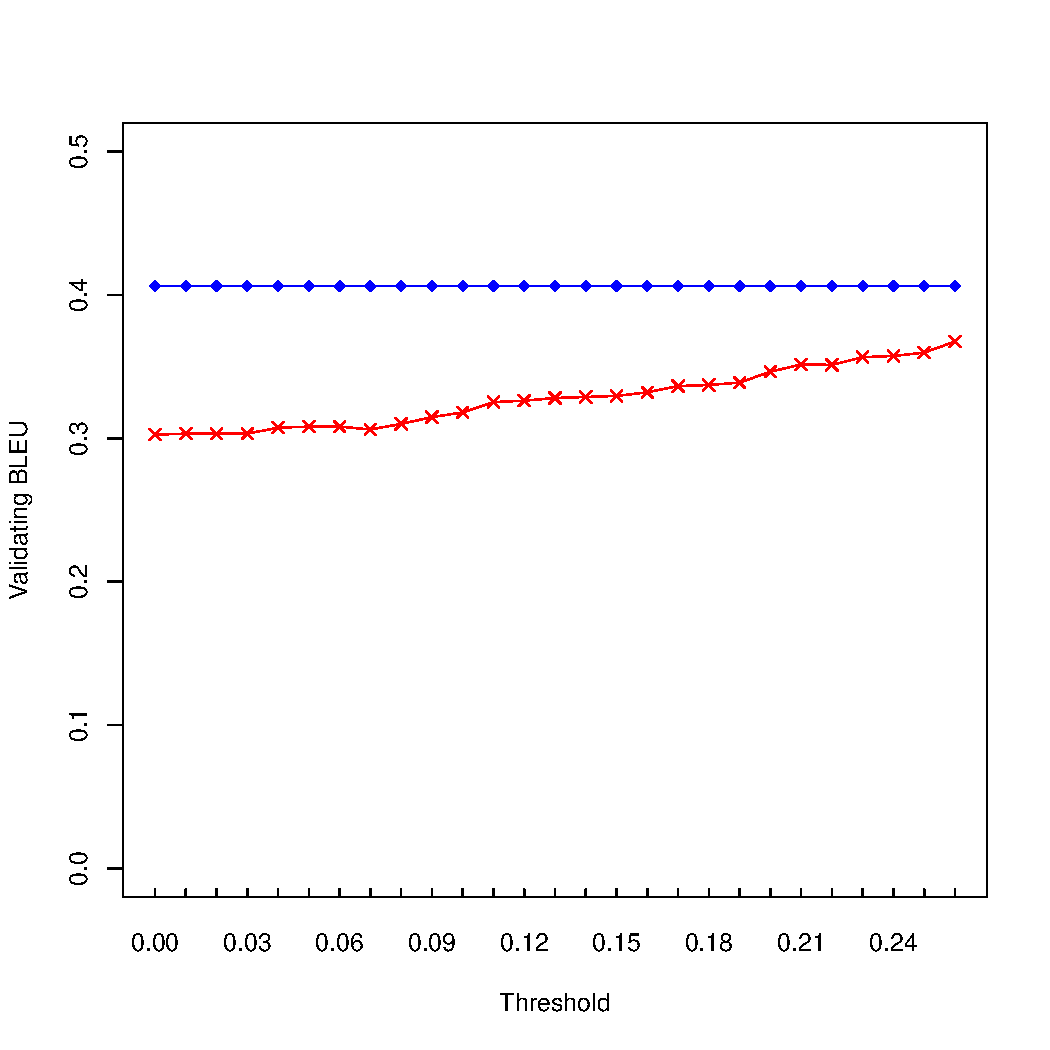
\includegraphics[width=\linewidth]{WorkerSelection/bleuthreshold.pdf}
%%  \caption{The Process to Sweep the Threshold}
%%    \label{fsweepthre}
%%\end{figure}
%
% We use each value  in the process  as the potential threshold.  We score translations of the foreign sentences in the validation set.  Since this approach assumes a temporal ordering of the translations, we compute the scores for each translation of a source sentence using the time-ordering of when Turkers submitted them. There are 2 conditions on the halt of this process for each foreign sentence: 1) the predicted BLEU score of some translation (submitted earlier than the last translation) is higher than the threshold or 2) we have scored all 4 translations.  
%
%%To evaluate the performance of the model running with different thresholds, we first compute an upper bound by selecting the best translation among all 4 candidates for each foreign sentence of the validation set according to our  model. We call this set $S_{upper}$.  $S_{upper}$ is the highest BLEU score we can get by choosing translation using the model, since it has access to all of the available translations.  
%
%After we have used the validation set to sweep various threshold values,  we can pick a suitable value for the threshold by picking the lowest value that is within some delta of $S_{upper}$, say  90$\%$. 
%
%Finally, we retrain our model using the union set of the training set and validation set, use the resulting model on the test set.  We evaluate the model's performance by counting the average number of candidate translations that it solicits per source sentence, and by computing the loss in overall BLEU score compared to when it had access to all 4 translations.  This evaluation shows how much money our model would save by eliminating unnecessary redundancy in the translation process, and how close it is to the upper bound on translation quality when using all of the translations from the original set.
%
%\subsection{Cost Savings}
%
%%"TODO:Here please write an analysis of how much money we could save if we choose some threshold for when we ask for a new translation.  Also, give an estimate of how much worse the translation quality is compared with keeping all of the workers."
%
%\begin{figure}[h!]
%  \centering
%  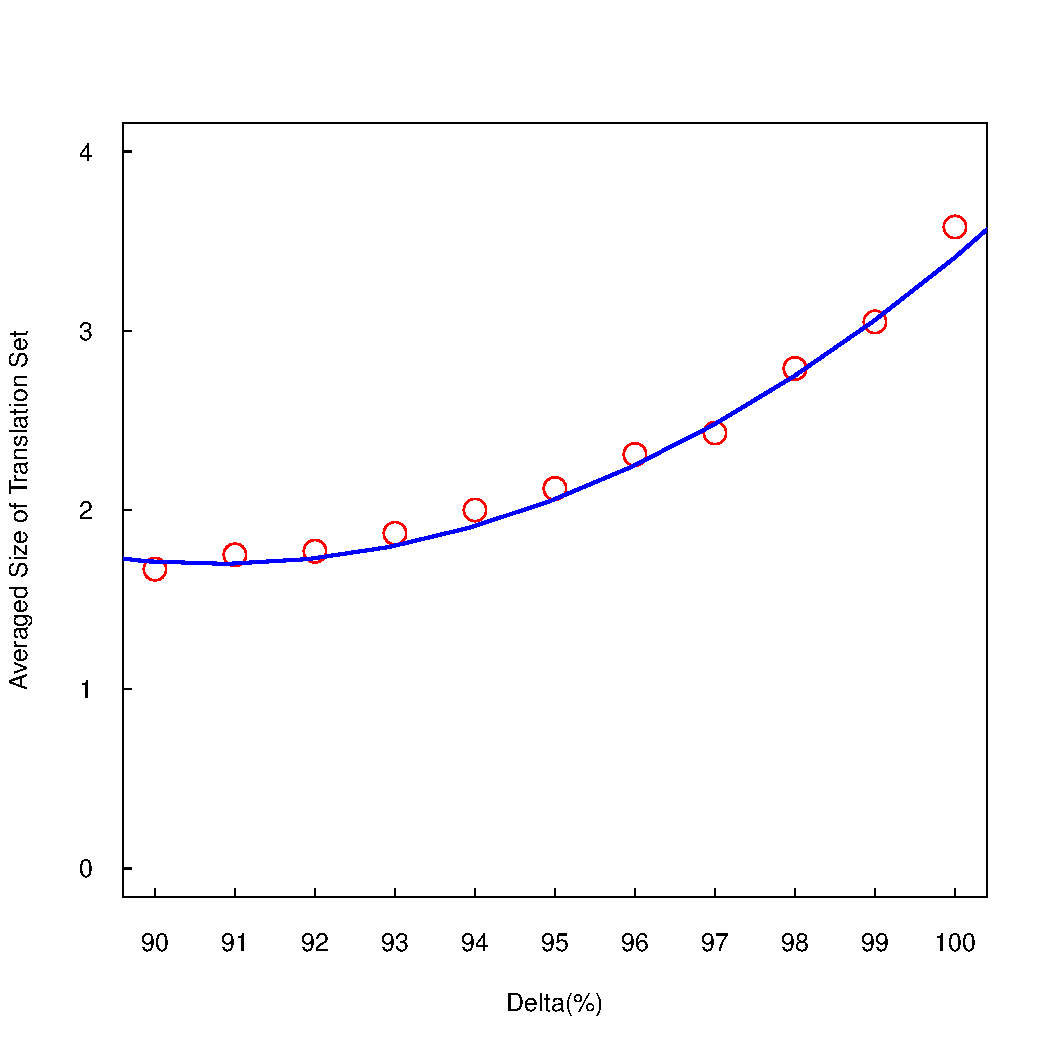
\includegraphics[width=\linewidth]{fitsizedelta/fit.pdf}
%  \caption{Relationship between \textit{delta} and \textit{\# of Trans}. Each red circle shows the \textit{delta} on x-axis and the average size of translation set on y-axis. The blue curve represents the model we fit to describe the relationship.}
%    \label{fit}
%\end{figure}
%
%From Table \ref{orderanother}, we see that the averaged size of translation sets is positive correlated to \textit{delta}. To analyze the cost saving more clearly, we fit a model to describe the relationship between \textit{delta} and \textit{\# of Trans}.Thus we can estimate the cost as a function of \textit{delta} which is the goal of  quality control, and bridge the gap between quality control and cost optimization.
%
%Figure \ref{fit} shows the relationship between \textit{delta} and \textit{\# of Trans}. The model we fit can be described as a function $f(x)$:
%\begin{align*}
%f(x) = 0.02x^2 - 3.63x+166.41
%\end{align*}
% where x is the value of \textit{delta}. The model fits the data pretty good and the average square error rate is 
%0.0054. Thus for a given value of \textit{delta} x, the cost is:
%\begin{align*}
%C& = 20\% \cdot N_{p}\cdot C_{p}  +  \frac{f(x)}{4}\cdot 80\% \cdot N_{np} \cdot C_{np}\\
%\end{align*} 
%
%\section{Discussion}
%
%%Crowdsourcing is attractive because it provides a way of creating translations at lower cost than hiring professional translators. 
%We have introduced several ways of lowering the costs associated with crowdsourcing translations:
%\begin{itemize}
%\item We show that we can quickly identify bad translators, either with a model designed to rank them, or by ranking them by having them first translate a small number of sentences with gold standard translations. The cost savings here comes from not hiring bad workers.
%\item After we have collected one translation of a source sentence, we consult a model that predicts whether its quality is sufficiently high or whether we should pay to have the sentence re-translated.  The cost savings here comes from reducing the number of redundant translations.
%\item In both cases we need a some amount of professionally translated materials  to use as a gold standard for calibration.  The cost of these professional translations can dominate the cost of our models, so we experiment with how little we can get away with.
%\end{itemize}
%In all cases, there is a trade-off between lowering our costs and producing high quality translations.  Figure \ref{fbleucost} plots the cost versus the BLEU scores for the different configurations that we experimented with.
%
%In Figure \ref{fbleucost}-(a) the increasing costs are a function of how many sentences we use to rank the translators.  Here we use no model, and simply rank the translators by their BLEU score against a small amount of gold standard data. The quality peaks at 37.9 BLEU after \$11,600.
%%the return on investment is low after spending the first \$2,000 to get a BLEU of 35.6.
%We are able to rank the translators with high accuracy and achieve a relative high BLEU score by paying for a comparatively small number of professional translations to use as calibration.   From our experiments,  10-20 professionally translated sentences seems like a reasonable number. 
%
%Figure\ref{fbleucost}-(b) uses a model to determine whether to purchase another translation.  Here the starting cost is high (nearly \$9,000) because the model requires a significant amount of professional translations in order to train the model and to determine the optimal threshold values for whether to solicit another translation. This model allows us to significantly improve the overall translation quality to a BLEU score of nearly 40, for a final cost of \$9,200.
%
%To emphasize the effectiveness of model selection approach, Figure \ref{fbleucost}-(c) plots the relationship between BLEU and non-professional component of the overall cost.  Past approaches to crowdsourcing translation always solicited 4 non-professional translations of every source sentence. The cost for translating our 1433 test sentences under this approach is \$573.44.  This produces the maximum BLEU score of 40.1.  Using our model to reduce the number of redundant translations, we can reduce the costs with mild degredation in translation quality.  We can cut the number of non-translations in half, and pay only \$286.72, while achieving a BLEU score of 37.6 (94\% of the maximum), or pay \$348.36,60.7\% of total non-professional translations' cost, for a BLEU of 38.5 (96\% of  the maximum).
%
%\begin{figure*}[htbp]
%  \centering
%  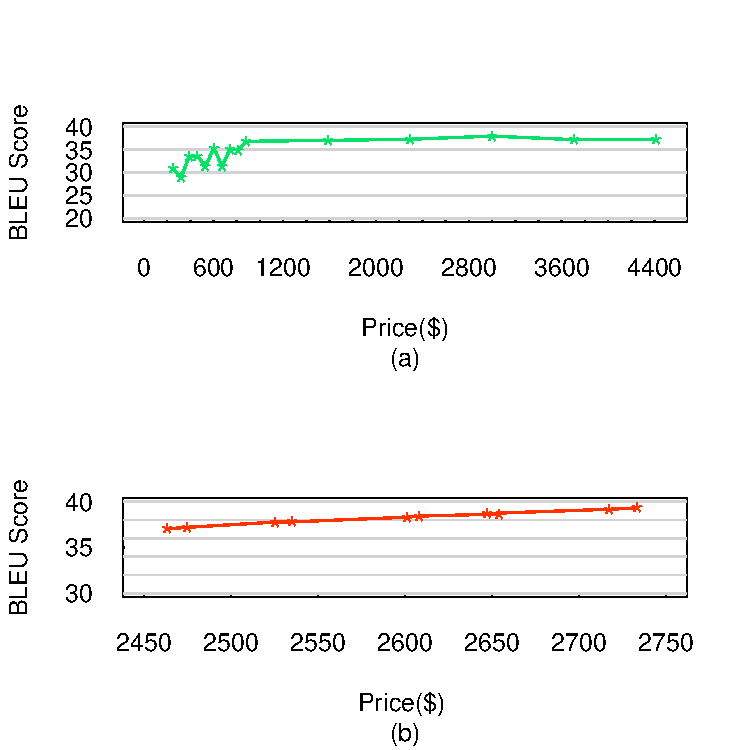
\includegraphics[width=\linewidth]{cost-bleu/pricecost.pdf}
%  \caption{The Relationship between BLEU score and costs. In Figure (a), the red line shows the relationship between BLEU score and  the total costs (professional and non-professional) for the ranking based approach. The green line shows the corresponding translation quality for gold standard ranking selection measured in BLEU score. Figure (b) shows the relationship between BLEU score and the total costs for model-based approach. Figure (c)  illustrates the relationship between BLEU score and non-professional costs for model based approach.}
%    \label{fbleucost}
%\end{figure*}
%
%
%\section{Related Work}
%%Crowdsoucing has been widely used in data annotation or labeling to get a large amount of data at low cost. The relationship between the budget and the quality was discussed in previous work.
%
%\cite{sheng2008get}'s work on repeated labeling presents a way of solving the problems of uncertainty in labeling. Since we cannot always get high-quality labeled data samples with relatively low costs in reality, to keep the model trained on noisy labeled data having a high accuracy in predicting, \newcite{sheng2008get} proposed a framework for repeated-labeling that resolves the uncertainty in labeling via majority voting. The experimental results show that a model's predicting accuracy is improved even if labels in its training data are nosity and of imperfect quality.  As long as the integrated quality (the probability of the integrated labeling being correct) is higher than 0.5, repeated labeling benefits model training. 
%
%\newcite{passonneau2013benefits} created a Bayesian model of annotation and they applied to the problem of word sense annotation. \newcite{passonneau2013benefits} also proposed an approach to detect and avoid spam workers. 
%%They required workers to finish 20000 HITs and have a 98\% lifetime approval rating. 
%They measured the performance of worker by comparing worker's labels to the current majority labels and worker with bad performance would be blocked. However, this approach suffered from 2 shortcomings: (1) Sometimes majority labels may not reflect the ground truth label. (2) They didn't figure out  how much data(HITs) is needed to evaluate a worker's performance. Although they could find the spam after the fact, it was a post-hoc analysis, so they had already paid for that worker and wasted the money.
%%More closer the quality to 0.5, the more benefits obtained in model prediction.
%%For one of our approaches for lowering the costs of crowdsourcing,  we train models to distinguish between acceptable and unacceptable translation candidates.  To do so,
%% Candidates with BLEU scores higher than the threshold are acceptable and vice versa. We search for the threshold on the validating set that is leading to the BLEU within some delta of $S_{upper}$.  
%%we sweep a threshold of BLEU values. The threshold between acceptable and unacceptable translations is fuzzy so there exists some uncertainty in labeling each data sample.  This is related to \cite{sheng2008get}'s work on repeated labeling, which presents a way of solving the problems of   uncertainty in labeling and selection of a threshold. In their work, they showed that for single-labeling examples, the labeling quality (the annotator's probability of producing a correct labeling) is critical to the model quality. The model prediction accuracy rises as the labeling quality increases. However, in reality, we cannot always get high-quality labeled data samples with relatively low costs. To keep the model trained on noisy labeled data having a high accuracy in predicting, \newcite{sheng2008get} proposed a framework for repeated-labeling that resolves the uncertainty in labeling via majority voting.  
%%The experimental results show that a model's predicting accuracy is improved even if labels in its training data are nosity and of imperfect quality.  As long as the integrated quality (the probability of the integrated labeling being correct) is higher than 0.5, repeated labeling benefits model training. More closer the quality to 0.5, the more benefits obtained in model prediction.
%
%%If we relax the condition on the uniform labeler quality and allow lablers to have different quality,  a new question arises: should we use the best individual labeler or should we combile the results from multiple labelers? According to the analysis,  it depends on how much the best labeler's quality is better the average quality of all labelers.
%
%%Majority voting is an useful approach to improve the quality of corpus. However, it omits  the uncertain property of data samples' labels and loses the information about uncertainty in labels. To take advantage of the uncertainty, \newcite{sheng2008get} represent labeling uncertainty in probability. For each unlabeled data sample $x_{i}$, the \textit{multiplied examples} (ME) procedure takes the existing multi-label set  $L_i = \{y_{ij}\}$ as input, and for each label value $y_{ij} $ in the multiset, make a replica of $x_i$ which is labeled $y_{ij}$, and use the probability of that label value appearing in the multi-label set as the weight of that replica . We can use cost-sensitive learning method to train model on the modified data set. Experiment shows that ME strategy is better than than majority voting.
%
%%In experiments, for each data set, 30\% data samples are held out as the test data, and the rest data is the "pool" from which we acquire unlabeled and labeled samples. When deciding the next data sample to be labeled, they use the generalized round robin strategy: selecting the data sample with the fewest labels. To make the selection more reasonable, they proposed the selective-repeated labeling method. For each data sample, $LU$ is defined as the label uncertainty which measures the labels' diversity on the data sample. Similarly, $MU$ is defined as the model uncertainty which measures the disagreement on models' prediction to the data sample. $LMU$ is defined as the label and model uncertainty which is the geometric average of $LU$ and $MU$. Instead of assigning the new label to  the data sample with fewest labels, they choose the data sample with the highest $LMU$ score and get benefits.
%
%%Outline of related work of 'Benefits of a Model of Annotation'.\\
%%1. Related Point: our work is trying to find the best translation from all candidates. Their work is trying to %select a label from the multi-label set.
%%2. Different Point: our work is don't have labels but they have.
%
%%A very important issue in natural language processing is data annotation. Hiring professional annotators is very expensive. As an alternative, collecting several annotation for each single data sample and pick the best label is  more economical.  In our work, we collected several translations for each source sentence and pick the best translation. Our work shares many goals in common with \newcite{passonneau2013benefits}, who created a Bayesian model of annotation, which they applied to the problem of word sense annotation. Rather than hiring professional annotators, which is very expensive, they hire non-expert annotators on Mechanical Turk.  They collected 20 to 25 word sense labels for each word. To decide which label to select for each word, and to compute the quality of the annotation, they proposed the probabilistic model using Bayes's rule. They calculated the product of the prior probability (the initial probability of being the observed label) and the conditional probability (the probability of being the observed label given the true label) and pick one label with the highest score. This sort of a probability estimate provides much more information about the corpus quality than previous methods, such as calculating inter-annotation agreement through Coehn's kappa score.  Kappa measures the agreement coefficient among annotators in a chance-adjusted fashion.  However, the method  only  reports how often annotators agree, but does not provide information about the quality of the corpus and the individual data sample.
%
%%Although \newcite{passonneau2013benefits} collect word sense labels, which are a small, enumerable set, and we collect translation (which could be thought of as a kind of label, albeit a very complex one), there is a strong commonality in the goals of their word and the goals of our work.  Specifically, how can we use all the labels collected in order to select of the best label.  And how can we rank the annotators themselves.  For selecting the best label for word senses, majority voting is a direct and easy way to solve the problem, but the task is more complex for translation. 
%
%%\newcite{passonneau2013benefits} also proposed an approach to detect and avoid spam workers. 
%%They required workers to finish 20000 HITs and have a 98\% lifetime approval rating. 
%%They measured the performance of worker by comparing worker's labels to the current majority labels and worker with bad performance would be blocked. However, this approach suffered from 2 shortcomings: (1) Sometimes majority labels may not reflect the ground truth label. (2) They didn't figure out  how much data(HITs) is needed to evaluate a worker's performance. Although they could find the spam after the fact, it was a post-hoc analysis, so they had already paid for that worker and wasted the money.  We attempt to identify poor workers as quickly as possible, in order to limit the amount of work that we solicit from them.
%\newcite{lin2014re} examined the relationship between worker accuracy and budget in the context of using crowdsourcing to train a machine learning classifier.  They show that if the goal is to train a classifier on the labels, that the properties of the classifier will determine whether it is better to re-label data (resulting in higher quality labels) or get more single labeled items (of lower quality). They showed that classifiers with weak inductive bias  benefit more from relabeling, and that relabeling is more important when worker accuracy is low (barely higher than 0.5). 
%Counter-intuitively, an infinite budget does not make relabeling work any better.
%
%\newcite{novotney2010cheap} showed a similar result for training an automatic speech recognition (ASR) system.  When creating training data for an ASR system, given a fixed budget. Their system's accuracy was higher when it is trained on more low quality transcription data compared to when it was trained on fewer high quality transcriptions.
%
%
%\section{Conclusion}
%In this paper, we propose two mechanisms to optimize cost: the ranking selection method and the model selection method. They have  different applicable scenarios. The ranking selection method is a very simple method without any model training. This approach is inspired by the intuition that workers' performance is consistent. The ranking selection method is suitable for crowdsourcing tasks which do not have specific requirements about the quality of the translations, or when the data collection is being performed by a requester who does not have sufficient background in machine learning in order to train a model, or when only very limited amounts of gold standard data are available.
%The model selection method works if there exists a specific requirement that the quality control must reach a certain threshold, or when more data needs to be collected.  This model is most effective when reasonable amounts of pre-existing professional translations are available for setting the models threshold.  Its major cost reduction comes from dramatically reducing the amount of non-professional data to maintain the same quality.
%\section*{Acknowledgments}
%
%Do not number the acknowledgment section. Do not include this section when submitting your paper for review.

\bibliographystyle{naaclhlt2015}
\bibliography{naaclhlt2015_new}

\end{document}